
\lhead{\emph{Quantification of AMC Prototype}}
%\part{Privacy Preserving Approximation of Edit Distance on Genomic Data}

\chapter{Quantification of AMC Prototype}\label{ch:quantification}
% \label{chap:image}

In Chapter~\ref{ch:operation}, the magnetic control process and the simulation methods to understand the process have been described. In addition to that for further quantification of the system some metrics have been defined. This chapter starts with the results following those metrics and side by side it also shows the results in terms of simulation methods. The chapter also includes some unique points which aren't explicitly present on previous studies on active compensation. Finally, it will end with some suggestions on fluxgate placements and effect of different shields. The new directions for future studies set by the unique points and the fluxgates placement's suggestions are presented in Chapter~\ref{ch:conclusion}.

% There are vast number of parameters that can be varied and studied for active compensation. For quantifying the the prototype, five among them are chosen based on importance, time limitation, resources available etc. and studied via both experiment and simulation. Those will create a huge impact for the future studies on active compensation. Some unique points have been discussed which aren't explicitly present on previous studies on active compensation. Their successfulness have been discussed using some metrics (see Section~\ref{sec:metrics}). In this chapter, studies on the parameter as well as the metrics to justify them will be discussed in terms of results.

\section{Sampling Frequency and Filtering}\label{sec:freq}


\begin{itemize}
\item We built some analog filters which were discussed in Chapter 3
\item Goal of the filter was to remove high-frequency noise (low-pass Butterworth with 10~Hz corner frequency)
\item This would allow the ADC to operate with less averaging, reducing its effective sampling time (denoted by the ``resolution index'')  (refer to Ch. 3)
\item We show the effectiveness in this section.
\end{itemize}

This Section talks about the sampling frequency and the effect of
filtering in sampling frequency. It starts with defining the sampling
frequency and how we first consider building an analog filter in the
first place. Then it shows the effect improving the response time on
the prototype. Finally, the Section wraps up with some comparison in
current response time for different sampling frequency.


Sampling frequency is the number of samples per second in a signal. For the prototype, by sampling frequency we meant that the number of signals of the fluxgate sensors that are going to the feedback algorithm via analog to digital converter (ADC) per second per measurement. But we are recording the time for a complete iteration which we call it as loop sampling frequency which includes the ADC sampling frequency plus rest of the loop frequency. In the early days of the prototype experiment, we have used the slowest sampling rate which is corresponding to resolution index 12 in Table~\ref{table:t7freq}.  The problem with that was the response time for the current was very slow and so does the compensation of the magnetic field. Then we have decided to use the fastest sampling frequency that the ADC can offer which is corresponding to resolution index 1 in Table~\ref{table:t7freq}. But new problem has arisen in terms of noise especially the 60 Hz electrical noise from the power source which has motivated us to build the 4\textsuperscript{th} order low pass Butterworth filter (see Section~\ref{sec:filter}) to get rid of unwanted high frequency noise. This Section talks about the results that we got to solve those problems by increasing the sampling frequency.

\subsubsection{Effect on Filtering to Use the Fastest Sampling Frequency}

\begin{itemize}
\item Fix Fig. 5.1 (scales) -- ideally plot all of them on the same graph.
\item Noise reduced by factor of {\bf X}
\item This is resolution index 1
\item Without filter noise is dominated by 60 Hz and higher.
\item Compensation is off
\item Also compared with SCU... it agreed well.  Our filters gave slightly better performance (lower noise) likely due to slight difference in design.
\item Loop frequency is 100~Hz.  This is larger than 25~kHz$/12\approx 2$~kHz reported in Chapter 3 (ref) because of polling time.  Typ.~1~ms/channel read.  When read in this way, can increase resolution index to 7 (and averaging time) before significant delays are noted.  (when ADC effective sample time approaches 1~ms)
\item At times we did this alternate way:  increase resolution index.
\item Another problem:  current drifting during compensation although field would not change.  This is discussed further in Sections~\ref{drifting1} and \ref{drifting2}.
\item We thought maybe this was due to sequential reads (higher resol index $\sim$ 7) so in general we aimed for resol index 1 which makes the reads distributed in time.  (Explain better... it is leading up to Fig. 5.2 and 5.3.)  In such cases when using lower resol index (1) we did software averaging until the design loop rate was met.  This will be discussed further in the next sections.
\item Another point:  in Fig. 5.1 is that there is a time lag (slewing?) for the filter... consistent with expectation.
\item Conclusion:  the filter works and allows us to go to higher effective sample rate.
\item We would be stuck at resolution index 11 or 12 otherwise.  12 has 6 Hz effective sample rate $\approx$ 10 PLC averaging.  If doing this for 12 channels it it means $<0.5$~Hz.  Impossible to do compensation at 6~Hz this way (fails to meet design goal).
\end{itemize}

As we have decided to use the fastest sampling frequency that our ADC
can offer as discussed above , we have faced problems in terms of
noise there. So, we have build a 4\textsuperscript{th} order low pass
Butterworth filter (see Section~\ref{sec:filter}) to get rid of
unwanted high frequency noise.

\fig{Images/filtering}{width = \textwidth}{Filtering effect on the data taken for magnetic field compensation. Vertical axis represent $\Delta$B (see Eq.~(\ref{eq:del_B})) due to '1y' . The left one indicates data measurement using a filter and right one without a filter. They are described more in the text. The 'ON' and 'OFF' vertical dashed lines indicate the time of the perturbation coil being turned 'ON' and 'OFF' respectively. \label{fig:filtering}}{Short}

The Fig.~\ref{fig:filtering} shows the importance of using the filter discussed above. The data was taken by measuring the drift in the signal $\Delta$B (see Eq.~(\ref{eq:del_B})) by '1y' sensor position two times where one with filter and another one without filter. On the part of data measurement, current has been applied in the perturbation coil at $\sim$ 0.18s which is indicated by the vertical red dashed line and is termed as ON. At $\sim$0.58s current supply in the perturbation coil has cut off which is indicated by the green vertical dash line and termed as OFF. The total loop sampling frequency is found to be 100 Hz. Now for comparison the data taken with filer has been shown in Fig.~\ref{fig:filtering}\textcolor{blue}{(a)} and that without filter in in Fig.~\ref{fig:filtering}\textcolor{blue}{(b)}. It is seen that the signal is very less attenuated while using filter and very noisy without any filter.

So, for faster sampling it needs to have filter to avoid high frequency noise. Next, after applying filter let's see how the sampling frequency has impact on response time of the magnetic field compensation.

%\FloatBarrier
\subsubsection{Effect on Response Time of Magnetic Field Compensation}

\begin{itemize}
\item Fig. 5.2.  Left: with filter, resol index 1, 50 software averages per point, compensation ON, loop cycle rate (correction rate) 6.57 Hz indicated in the Fig.  Right:  no filter, resolution index 12, no other averaging (other than what the ADC oes), graph is on longer timescale because loop rate is slower (0.45~Hz).  Corrected/uncorrected (projected) values are shown.
\item Main point:  loop cycle rate is good!  $\sim$ 15x faster.  Even plenty of time for additional averaging to reduce noise further.  Likely the same result if somewhat higher resolution index used, possibly even with reduced software averaging.
\end{itemize}




So after we have our filter ready to use, now let's see what I meant by increasing the sampling frequency and its effect on the magnetic field  compensation response time.

\fig{Images/samp_freq_iteration}{width = \textwidth}{Active magnetic field compensation by sensor position '1y'. Vertical axis represent $\Delta$B (see Eq.~(\ref{eq:del_B})) due to '1y' with red represents uncompensated $\Delta$B. The left one indicates the compensation by '1y' at the fastest sampling frequency and right one for slowest one. They are described more in the text. The 'ON' and 'OFF' vertical dashed lines indicate the time of the perturbation coil being turned 'ON' and 'OFF' respectively. \label{fig:samp_freq_iteration}}{Short}

The Fig.~\ref{fig:samp_freq_iteration} shows the comparison between using highest sampling frequency (left) and the slowest one (right). The results are part of the compensation by all the 12 sensors placed just like explained by the horizontal axis in Fig.~\ref{fig:m} using regularized pseudinverse and PI tuning in the feedback algorithm explained in Chapter~\ref{ch:operation}. The figure only shows compensation for position '1y for simplicity. Note that the left and right are two different compensation measurements wih highest and lowest sampling frequency of our ADC (see Section~\ref{sec:DAQ}) having same number of feedback loop in each case. It is seen that for same number of measurements in the feedback algorithm it takes $\sim$45 s for the fastest one (left) compared to $\sim$670 s for the slowest one (right). The loop sampling  frequency for the fastest one (left) is 6.57 Hz compared to 0.45 Hz (left) for the slowest one (right). 

So the fastest sampling frequency of our ADC can offer 670/45$\approx$15 times faster response time than the slowest one. Next let's reveal the effect of sampling frequency on coil current response time.

%\FloatBarrier
\subsubsection{Effect on Coil Current Response Time }

\begin{itemize}
\item Fig. 5.3.  Always filtered.  Different resolution indices indicated on the figure along with their loop cycle rates.  Always 50 software averages done.
\item By resolution index 8 or 9, the loop cycle rate for the 50 software averages slows to 1.1 and 0.39 Hz respectively.  The results look similar to resolution index 12 (without filter) but much less noisy, smoother.
\item 
\end{itemize}


Form above discussion it is found that the more the sampling frequency is the less it takes for the compensation to respond. The effect of the sampling frequency has been revisited here again to show its effect in coil current response time.

\FloatBarrier
\fig{Images/samp_freq_example}{width = \textwidth}{$C_x^-$ coil current (left) and active magnetic field compensation (right) by sensor position '8x' for different resolution index. The resolution indices are (see Table~\ref{fig: res} and Sec.~\ref{sec:DAQ}) represented by 1, 6, 7, 8 and 9 while loop sampling frequencies are given in the parentheses respectively. They are describe more in the text. Vertical axis of the left one represents $C_x^-$ coil current graph and the right one indicates   $\Delta$B (see Eq.~(\ref{eq:del_B})) due to '8x' with red represents uncompensated $\Delta$B for different resolution index respectively. The 'ON' and 'OFF' vertical dashed lines indicate the time of the perturbation coil being turned 'ON' and 'OFF' respectively. \label{fig:samp_freq_example_multi}}{Short}

 The effect in coil current response time has been shown by Fig.~\ref{fig:samp_freq_example_multi}.  The results are again part of the compensation by all the 12 sensors placed just like explained earlier. Only difference here is that, now the different measurements have been taken for a same time frame i.e. 180s in this case compared to earlier where time was independent for different ones. For simplicity only $C_x^-$ coil current (left) and magnetic compensation (right) on fluxgate sensor position '8x' for different loop sampling frequencies have been shown instead of showing all current coils and sensor positions. For a complete list of positions see the color map of $\bm{M}$ in Fig.~\ref{fig:m}. As seen from the $C_x^-$ coil current (left) and $\Delta$B (right) due to '8x' graph that with decrease of loop sampling frequency, the current response time increases. For example, it takes $\sim$ 7s for $C_x^-$ coil current to settle down after the perturbation coil being turned ON when the loop sampling frequency is 6.35 Hz indicated by blue color curve compared to $\sim$ 52s when the loop sampling frequency is 0.39 Hz indicated by magenta color curve. So, the current response time has been faster by 52/7$\approx$7.5 times and we are not even considering the slowest one.

So for better response time in the coil current and eventually in magnetic field compensation system, there should an ADC with higher sampling frequency and a filtering method to get rid of higher frequencies. In the upcoming Section PI, regularization parameter and condition number will be revisited with results.

\section{Regularization Parameter and PI Tuning Revisited}
This Section starts with the reconstruction of the Fig.~\ref{fig:Isim}, Fig.~\ref{fig:fluc-sim} and Fig.~\ref{fig:I-fluc} in the experimental environment to justify the Monte Carlo simulation to find regularization parameter 'r' discussed on Section~\ref{sec:mont}. In Section~\ref{sec:tune}, tuning method of proportional gain (P) or $k_c^p$ term  and integral reset (I) or $k_c^i$ term (
see Eq.~(\ref{eq:I}) ) which is in short PI tuning has been discussed. After justifying 'r', in this Section, the discussion about the effect of changing P and I term individually will be made and then ended with discussing the effect of applying them combinely. The results of each of the effects will be presented and discussed.


\subsection{Justification of Monte Carlo Simulation to Find r}

In Section~\ref{sec:inv}, we have already talked about how the regularization parameter 'r' came into effect. Then, in Section~\ref{sec:mont}, a Monte Carlo simulation method has been described which has been taken from Ref.~\cite{bea} where a suitable value of 'r' has been found which will give the best compromise between the magnetic field fluctuation and coil current fluctuation. In this Section, we have run the model in experimental setup in order to verify the simulation method.

In Section~\ref{sec:mont}, 30 different sets of random magnetic field ($B_s^{\text{rand}}$) values have been chosen with center of distribution being 0 and standard deviation 5 nT for 12 different fluxgate sensor positions whose labels are given in the horizontal axis of Fig.~\ref{fig:m} and the positions are specified in Fig.~\ref{fig: coil}. Here, we have chosen one out of the 30 different sets of $B_s^{\text{rand}}$ and go through the steps as in Section~\ref{sec:mont} to generate similar figures like in Fig.~\ref{fig:Isim}, Fig.~\ref{fig:fluc-sim} and Fig.~\ref{fig:I-fluc}. For the experimental setup, we have done the similar steps to generate those figures except instead of generating $B_s^{\text{rand}}$ randomly, we have applied current in the perturbation coil to generate the required drift ( see Eq.~(\ref{eq:del_B}) ) which will be treated as $B_s^{\text{rand}}$. The results of the simulation as well as experiment are given in Fig.~\ref{fig:mont_comp}, where Fig.~\ref{fig:mont_comp}\textcolor{blue}{(a)}, Fig.~\ref{fig:mont_comp}\textcolor{blue}{(b)} and Fig.~\ref{fig:mont_comp}\textcolor{blue}{(c)} are the results found from simulation and Fig.~\ref{fig:mont_comp}\textcolor{blue}{(d)}, Fig.~\ref{fig:mont_comp}\textcolor{blue}{(e)} and Fig.~\ref{fig:mont_comp}\textcolor{blue}{(f)} are the results found from experiment. They are described in detail in Fig.~\ref{fig:Isim}, Fig.~\ref{fig:fluc-sim} and Fig.~\ref{fig:I-fluc}. It is seen that the experimental counterpart of each of the simulation that is Fig.~\ref{fig:mont_comp}\textcolor{blue}{(a)} of simulation is comparable to Fig.~\ref{fig:mont_comp}\textcolor{blue}{(d)} of experiment. Similarly, Fig.~\ref{fig:mont_comp}\textcolor{blue}{(b)} of simulation with Fig.~\ref{fig:mont_comp}\textcolor{blue}{(e)} of experiment and Fig.~\ref{fig:mont_comp}\textcolor{blue}{(c)} of simulation with Fig.~\ref{fig:mont_comp}\textcolor{blue}{(f)} of experiment are comparable and they produce similar results. The similar results of the simulation with experiment justifies the the simulation model described in Section~\ref{sec:mont}.

\fig{Images/mont_comp2}{width = \textwidth,height =10cm}{Simulation result for one set of $B_s^{\text{rend}}$ for the Fig.~\ref{fig:Isim}, Fig.~\ref{fig:fluc-sim} and Fig.~\ref{fig:I-fluc} are shown in (a), (b) and (c) and corresponding experimental results are in (d), (e) and (f). For the description of the figures see the text in Fig.~\ref{fig:Isim}, Fig.~\ref{fig:fluc-sim} and Fig.~\ref{fig:I-fluc}. For position of fluxgate sensors see Fig.~\ref{fig: coil}.\label{fig:mont_comp}}{Short}

\FloatBarrier
The above results in Fig.~\ref{fig:mont_comp}, where simulation results are similar to experimental one justify the simulation method described in Section~\ref{sec:mont}. The upcoming Section is all about P and I term (see Eq.~(\ref{eq:I}) ) behaviour. 

\subsection{PI Tuning General Behavior}\label{sec:pi_behave}
Here, the individual effect of P and I term will be discussed first and then concludes with the effect of using PI together.

\subsubsection{Effect of changing only P term}
Here, the effect of changing proportional gain term (P) or $k_c^p$ of Eq.~(\ref{eq:I}) will be discussed.

P term is proportionally multiplying the error (the difference between setpoint and actual measurement) with a constant gain. For the prototype it is

\begin{equation}
    P_{\text{PI}}=k_c^p \Delta I_c^n
\end{equation}
where, $k_c^p$ is the proportional gain and $\Delta I_c^n$ is explained in Eq.~(\ref{eq:del_I}).

Depending on the value $k_c^p$, it tries to minimize the error level between the setpoint and the actual measurement with passage of several measurements. A large value of $k_c^p$ will result large output change for a particular error and eventually it reaches a threshold point above which the system becomes unstable. 

% \begin{figure}[!htb]
%     \begin{subfigure}{.5\linewidth}
%         \centering
%         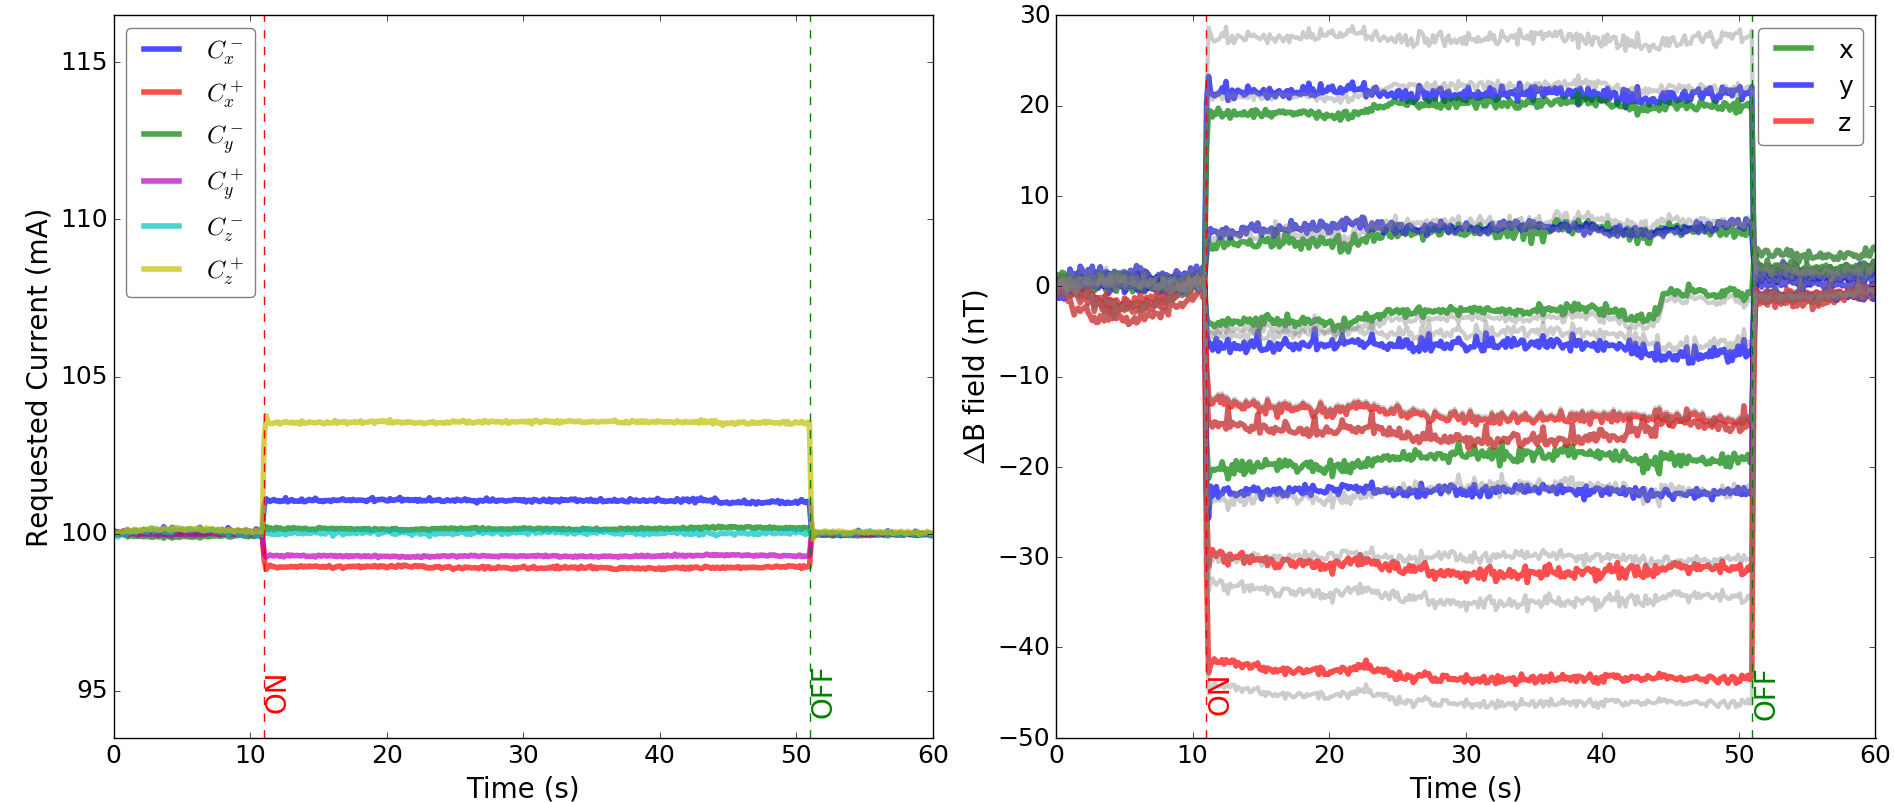
\includegraphics[width=\linewidth, height= 6.5 cm]{Images/p25}
%         \caption{at $k_c^p$=0.25}
%         \label{fig:p25}
%     \end{subfigure}%
%     \begin{subfigure}{.5\linewidth}
%         \centering
%         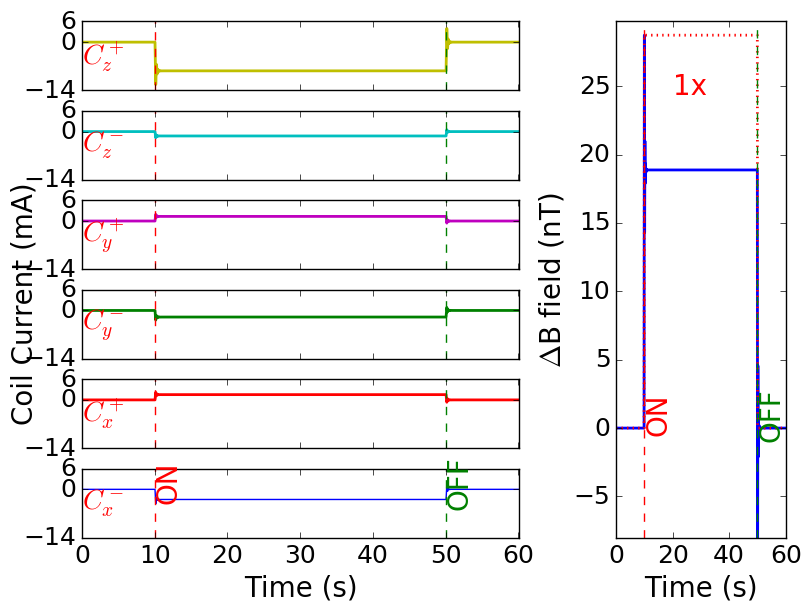
\includegraphics[width=\linewidth, height= 6.5 cm]{Images/p50}
%         \caption{at $k_c^p$=0.50}
%         \label{fig:p50}
%     \end{subfigure}\\[1ex]
%     \begin{subfigure}{.5\linewidth}
%         \centering
%         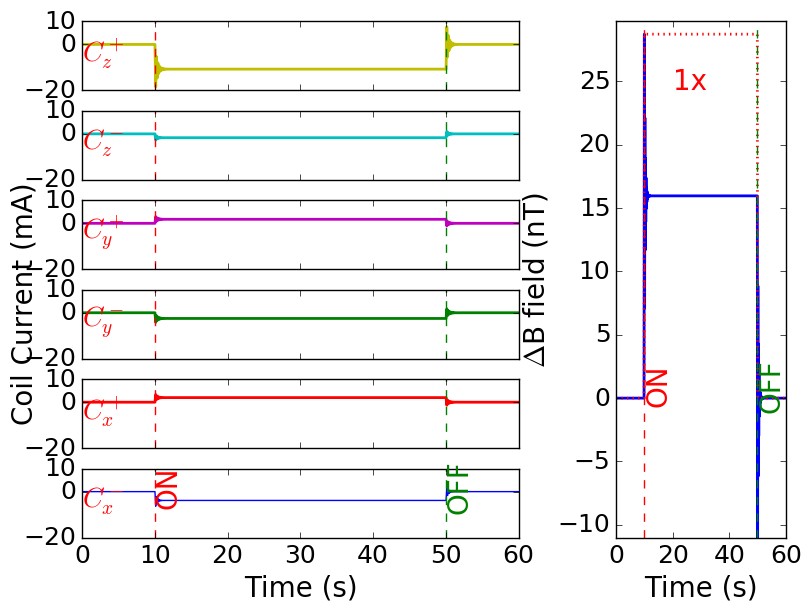
\includegraphics[width=\linewidth, height= 6.5 cm]{Images/p75}
%         \caption{at $k_c^p$=0.75}
%         \label{fig:p75}
%     \end{subfigure}%
%         \begin{subfigure}{.5\linewidth}
%         \centering
%         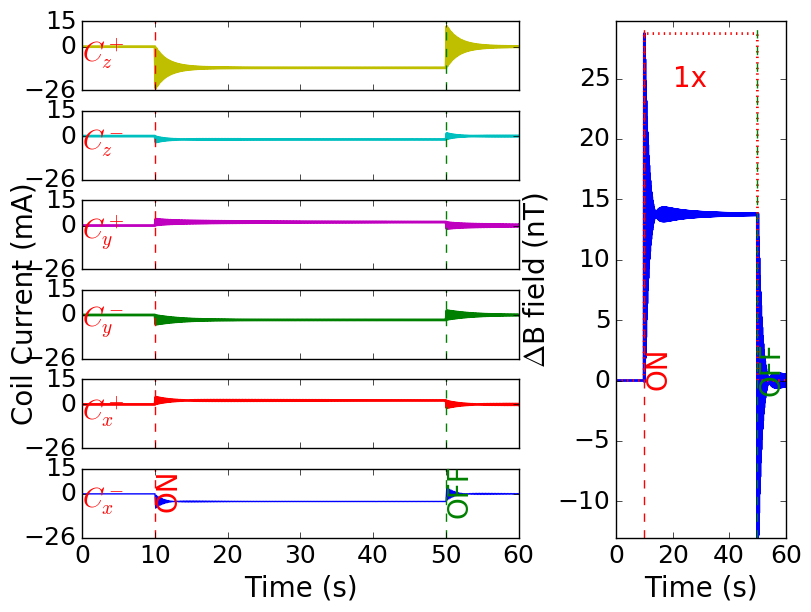
\includegraphics[width=\linewidth, height= 6.5 cm]{Images/p100}
%         \caption{at $k_c^p$=1.0}
%         \label{fig:p100}
%     \end{subfigure}

%     \caption{Currents (left vertical axis) in all six coil sides ($C_x^\pm$, $C_y^\pm$ and $C_z^\pm$) with drift $\Delta$B (right vertical axis) at sensor position '1x' for different values of $k_c^p$ with $k_c^i$ in Eq.~(\ref{eq:I}) being zero. Blue color curve denotes the actual drift in signal at position '1x' found by Eq.~(\ref{eq:del_B}) while the red curve denotes the drift that would have been without the compensation. The 'ON' and 'OFF' vertical dashed lines indicate the time of the perturbation coil being turned 'ON' and 'OFF' respectively. For position of coils and sensors see Fig.~\ref{fig: coil}. }
%     \label{fig:p_pi}
% \end{figure}
\begin{figure}[!htb]
    \begin{subfigure}{.5\linewidth}
        \centering
        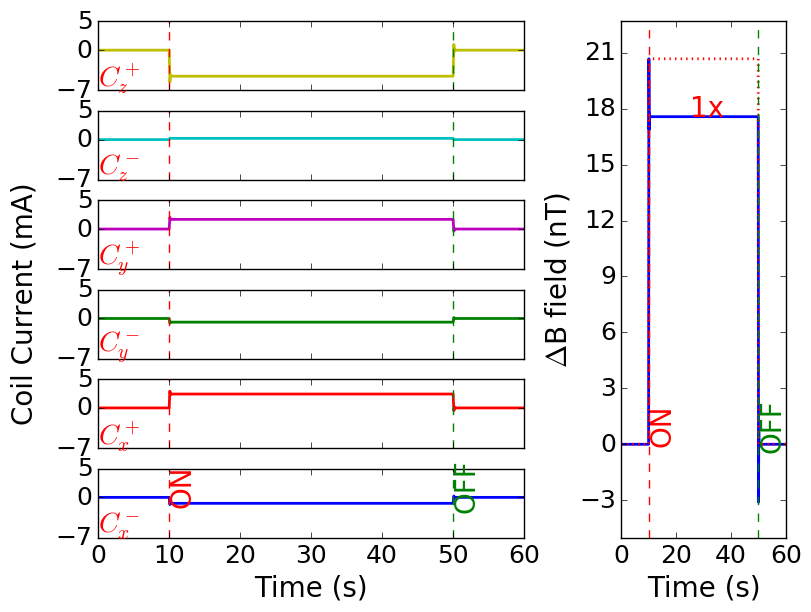
\includegraphics[width=\linewidth, height= 6.5 cm]{Images/p25_33}
        \caption{at $k_c^p$=0.25}
        \label{fig:p25}
    \end{subfigure}%
    \begin{subfigure}{.5\linewidth}
        \centering
        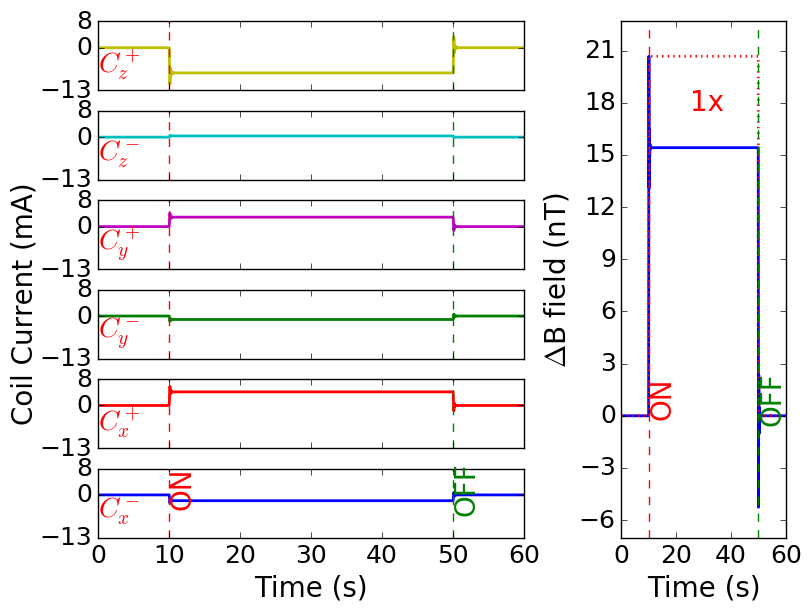
\includegraphics[width=\linewidth, height= 6.5 cm]{Images/p50_33}
        \caption{at $k_c^p$=0.50}
        \label{fig:p50}
    \end{subfigure}\\[1ex]
    \begin{subfigure}{.5\linewidth}
        \centering
        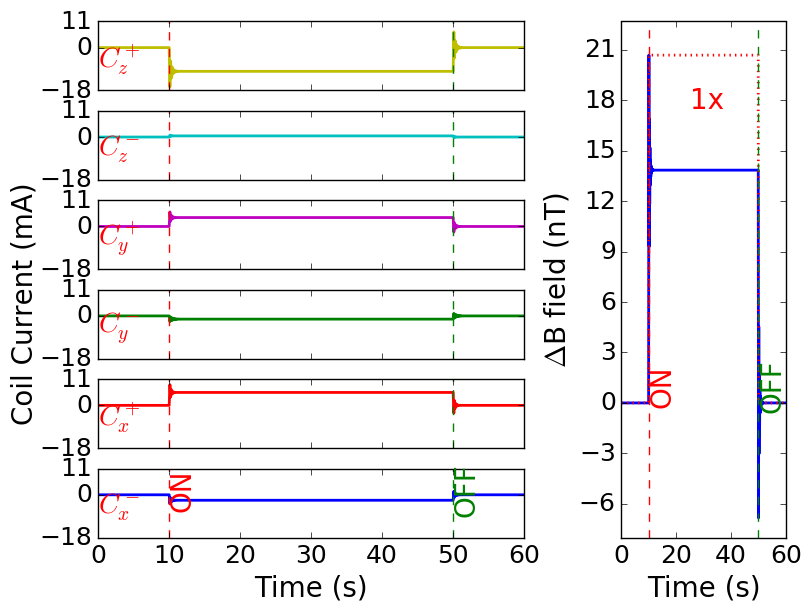
\includegraphics[width=\linewidth, height= 6.5 cm]{Images/p75_33}
        \caption{at $k_c^p$=0.75}
        \label{fig:p75}
    \end{subfigure}%
        \begin{subfigure}{.5\linewidth}
        \centering
        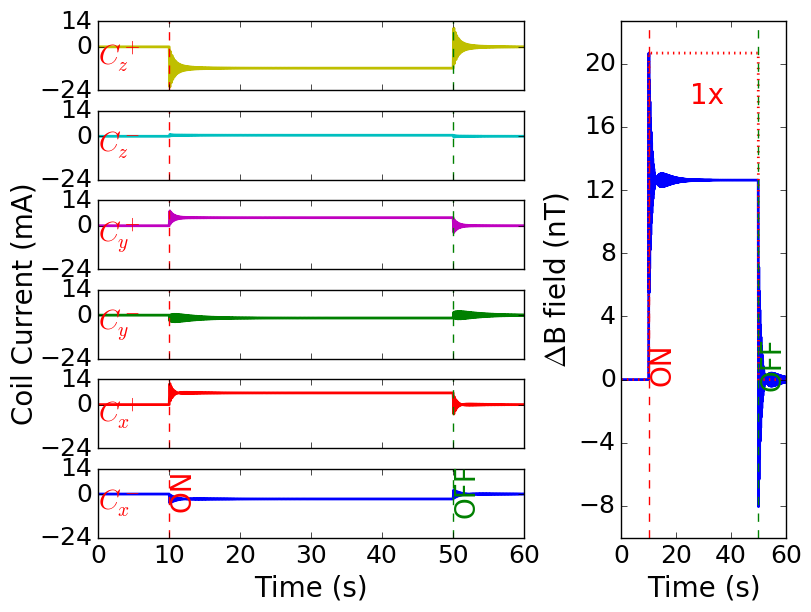
\includegraphics[width=\linewidth, height= 6.5 cm]{Images/p100_33}
        \caption{at $k_c^p$=1.0}
        \label{fig:p100}
    \end{subfigure}

    \caption[short]{Currents (left vertical axis) in all six coil sides ($C_x^\pm$, $C_y^\pm$ and $C_z^\pm$) with drift $\Delta$B (right vertical axis) at sensor position '1x' for different values of $k_c^p$ with $k_c^i$ in Eq.~(\ref{eq:I}) being zero. Blue color curve denotes the actual drift in signal at position '1x' found by Eq.~(\ref{eq:del_B}) while the red curve denotes the drift that would have been without the compensation. The 'ON' and 'OFF' vertical dashed lines indicate the time of the perturbation coil being turned 'ON' and 'OFF' respectively. For position of coils and sensors see Fig.~\ref{fig: coil}. }
    \label{fig:p_pi}
\end{figure}

The effect of changing $k_c^p$ has been shown in Fig.~\ref{fig:p_pi} where the currents (left) that are being sent to the coils ($C_x^\pm$, $C_y^\pm$ and $C_z^\pm$) for drift $\Delta$B found by Eq.~(\ref{eq:del_B}) in sensor position '1x'.  It is seen that $\Delta$B=17.5 nT, 15.5 nT and 13.5 nT for $k_c^p$ = 0.25, 0.5 and 0.75 respectively (see Fig.~\ref{fig:p_pi}\textcolor{blue}{(a)}, Fig.~\ref{fig:p_pi}\textcolor{blue}{(b)}, Fig.~\ref{fig:p_pi}\textcolor{blue}{(c)}). That is, with the increase of $k_c^p$, $\Delta$B magnetic field decreases. But, it has a limit after which with the increase of $k_c^p$, the systems becomes unstable and starts oscillating which can be seen from Fig.~\ref{fig:p_pi}\textcolor{blue}{(d)}) where the currents (left) are oscillating and the drift itself also at $\Delta$B=12.5 nT (right). So, the error is reduced maximum by (20.5-12.5)/20.5 * 100$\%\approx$37$\%$ from the initial drift of $\Delta$B=20.5 nT denoted by the red curve at position '1x'. 

\FloatBarrier
The above results confirm that the difference between the setpoint and the actual measurements of the magnetic field can be reduced upto a certain point. So, only having the P term is no the solution for the prototype. Next, we will discuss about the effect of only I term.

\subsubsection{Effect of changing only I term}
Here, the effect of changing integral reset term (I) or $k_c^i$ of Eq.~(\ref{eq:I}) will be discussed.

The error (the difference between setpoint and actual measurement) is accumulated for the length of measurements and I term is multiplying that accumulated error  with a constant gain. For the prototype it is

\begin{equation}
    I_{\text{PI}}=k_c^i \sum_n \Delta I_c^n
\end{equation}
where, $k_c^i$ is the integral gain and $\Delta I_c^n$ is explained in Eq.~(\ref{eq:del_I}).

Accumulated error keep tracks of the offsets that should be corrected previously. I term takes care of the offset which are not corrected by the P term and thus accelerates reducing the error level. Depending on the value $k_c^i$, how fast the feedback loop will response to the drift in the signal will be determined. A large value of $k_c^p$ will result large faster response to reducing the error level and eventually it reaches a threshold point above which the actual measurement will overshoot i.e. exceed the setpoint. 
% The main downfall of this is that the time required for the coil current to be settle in after reducing the error level may be very slow or never ever settle in.



% As like the effect on P, the effect of changing I has been shown in Fig.~\ref{fig:i_pi} where the change in current in all six coil sides with  $\Delta$B on a particular sensor position have been observed for $k_c^i$=0.25, 0.5, 0.75 and 1.0 . It is seen that with increase of I the level of compensation of the magnetic field is almost similar but the main difference occurs on how fast the system response in an expense of increasing current in all the coil sides (see Fig.~\ref{fig:i_pi}\textcolor{blue}{(a)}, Fig.~\ref{fig:i_pi}\textcolor{blue}{(b)}, Fig.~\ref{fig:i_pi}\textcolor{blue}{(c)} and Fig.~\ref{fig:i_pi}\textcolor{blue}{(d)}). The main problem with changing only I term is that it creates a very slow current response time. But, in terms of compensation only changing I gives very good result. The slow current response can be minimized by decreasing the value of optimized 'r' (see Section~\ref{sec:r_pi} and Section~\ref{sec:r_currentResponse} ).

% \begin{figure}[!htb]
%     \begin{subfigure}{.5\linewidth}
%         \centering
%         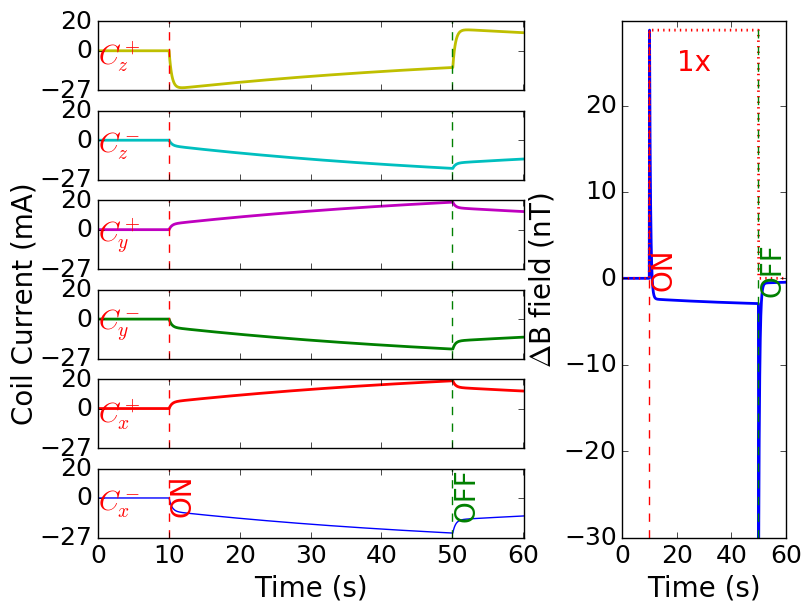
\includegraphics[width=\linewidth, height= 6.5 cm]{Images/i25}
%         \caption{at $k_c^i$=0.25}
%         \label{fig:i25}
%     \end{subfigure}%
%     \begin{subfigure}{.5\linewidth}
%         \centering
%         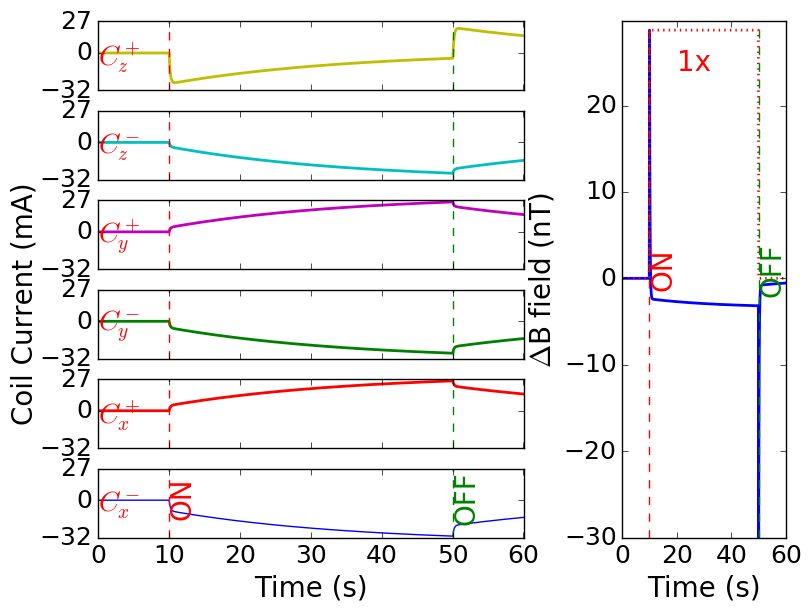
\includegraphics[width=\linewidth, height= 6.5 cm]{Images/i50}
%         \caption{at $k_c^i$=0.5}
%         \label{fig:i50}
%     \end{subfigure}\\[1ex]
%     \begin{subfigure}{.5\linewidth}
%         \centering
%         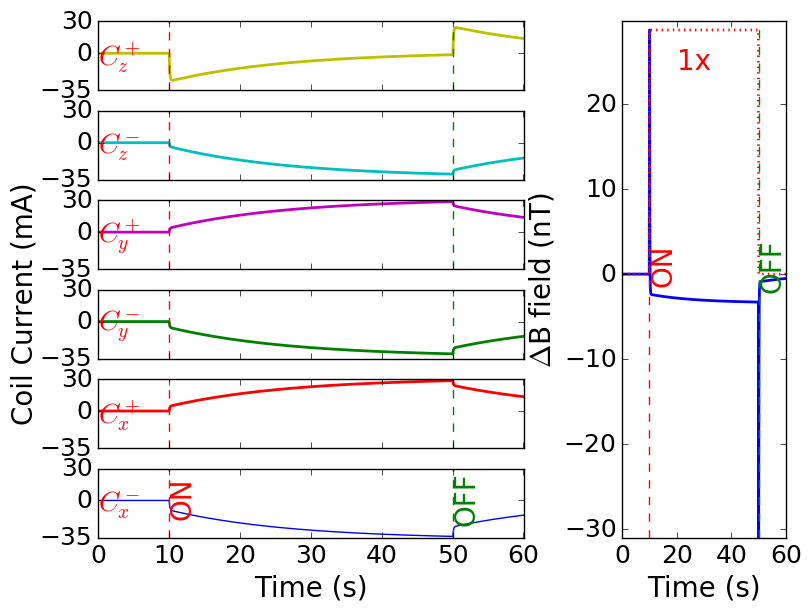
\includegraphics[width=\linewidth, height= 6.5 cm]{Images/i75}
%         \caption{at $k_c^i$=0.75}
%         \label{fig:i75}
%     \end{subfigure}%
%         \begin{subfigure}{.5\linewidth}
%         \centering
%         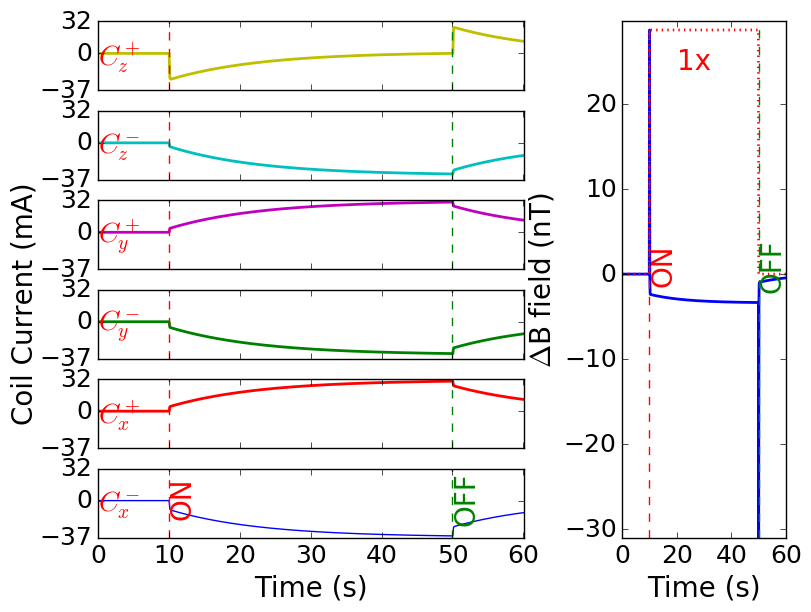
\includegraphics[width=\linewidth, height= 6.5 cm]{Images/i100}
%         \caption{at $k_c^i$=1.0}
%         \label{fig:i100}
%     \end{subfigure}

%     \caption{Currents (left vertical axis) in all six coil sides ($C_x^\pm$, $C_y^\pm$ and $C_z^\pm$) with drift $\Delta$B (right vertical axis) at sensor position '1x' for different values of $k_c^i$ with $k_c^p$ ( see Eq.~(\ref{eq:I}) ) being zero. Blue color curve denotes the actual drift in signal at position '1x' found by Eq.~(\ref{eq:del_B}) while the red curve denotes the drift that would have been without the compensation. The 'ON' and 'OFF' vertical dashed lines indicate the time of the perturbation coil being turned 'ON' and 'OFF' respectively. For position of coils and sensors see Fig.~\ref{fig: coil}.}
%     \label{fig:i_pi}
% \end{figure}
\begin{figure}[!htb]
    \begin{subfigure}{.5\linewidth}
        \centering
        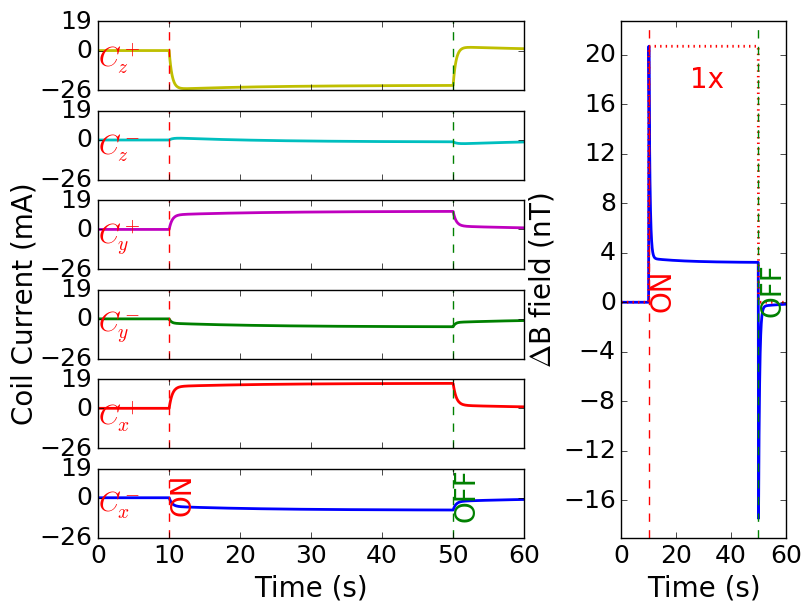
\includegraphics[width=\linewidth, height= 6.5 cm]{Images/i25_33}
        \caption{at $k_c^i$=0.25}
        \label{fig:i25}
    \end{subfigure}%
    \begin{subfigure}{.5\linewidth}
        \centering
        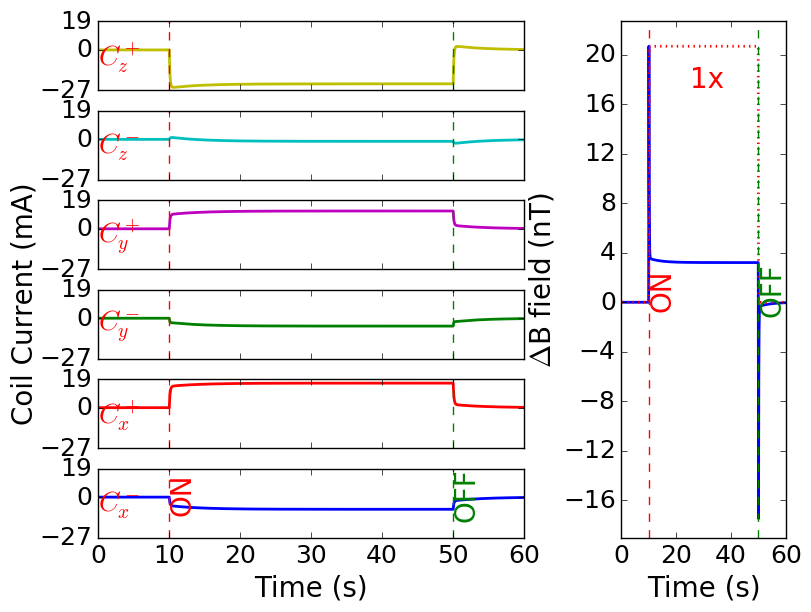
\includegraphics[width=\linewidth, height= 6.5 cm]{Images/i75_33}
        \caption{at $k_c^i$=0.75}
        \label{fig:i50}
    \end{subfigure}\\[1ex]
    \begin{subfigure}{.5\linewidth}
        \centering
        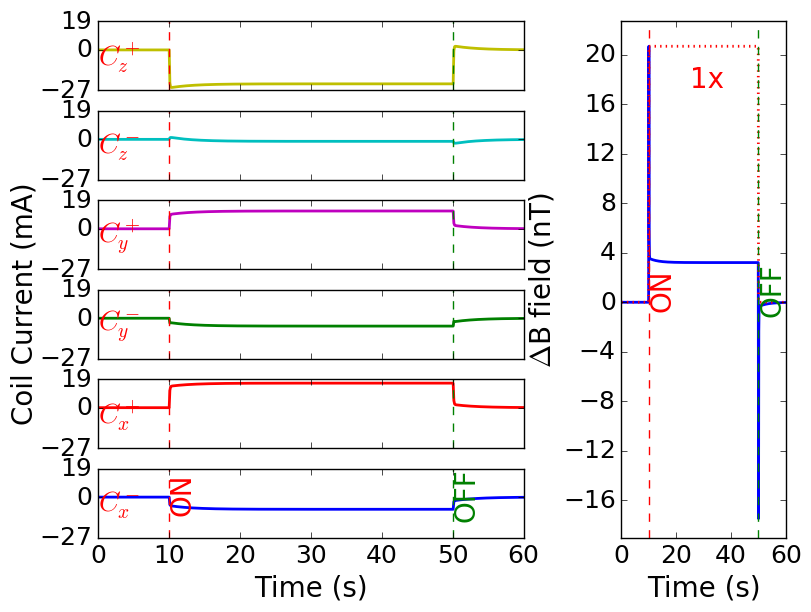
\includegraphics[width=\linewidth, height= 6.5 cm]{Images/i100_33}
        \caption{at $k_c^i$=1.0}
        \label{fig:i75}
    \end{subfigure}%
        \begin{subfigure}{.5\linewidth}
        \centering
        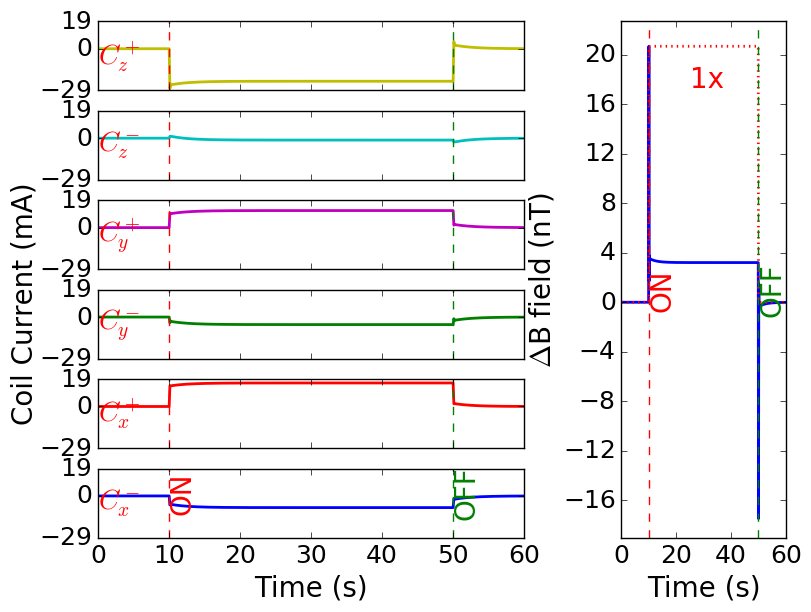
\includegraphics[width=\linewidth, height= 6.5 cm]{Images/i125_33}
        \caption{at $k_c^i$=1.25}
        \label{fig:i100}
    \end{subfigure}

    \caption[short]{Currents (left vertical axis) in all six coil sides ($C_x^\pm$, $C_y^\pm$ and $C_z^\pm$) with drift $\Delta$B (right vertical axis) at sensor position '1x' for different values of $k_c^i$ with $k_c^p$ ( see Eq.~(\ref{eq:I}) ) being zero. Blue color curve denotes the actual drift in signal at position '1x' found by Eq.~(\ref{eq:del_B}) while the red curve denotes the drift that would have been without the compensation. The 'ON' and 'OFF' vertical dashed lines indicate the time of the perturbation coil being turned 'ON' and 'OFF' respectively. For position of coils and sensors see Fig.~\ref{fig: coil}.}
    \label{fig:i_pi}
\end{figure}

\FloatBarrier
The effect of changing $k_c^i$ has been shown in Fig.~\ref{fig:i_pi} where the currents (left) that are being sent to the coils ($C_x^\pm$, $C_y^\pm$ and $C_z^\pm$) for drift $\Delta$B found by Eq.~(\ref{eq:del_B}) in sensor position '1x'.  It is seen from Fig.~\ref{fig:i_pi}\textcolor{blue}{(a)}, Fig.~\ref{fig:i_pi}\textcolor{blue}{(b)}, Fig.~\ref{fig:i_pi}\textcolor{blue}{(c)} and Fig.~\ref{fig:i_pi}\textcolor{blue}{(d)} which are correspond to $k_c^i$ = 0.25, 0.75, 1.0 and 1.25 respectively that the error level (right) seems to be $\sim$3.5 nT in every case and the coil currents(left) settle  faster for increasing value of $k_c^i$. The figures are neither helpful to understand the system response time nor the overshoot effect in the $\Delta$B graph (right). So for understating those effects, the $\Delta$B graphs (right) have been zoomed in and shown in Fig.~\ref{fig:i_pi_zoom}. Now it is easily seen that for the same duration of perturbation (here 'ON' at 10s and 'OFF' at 50s and so total 40s), the system still correcting the error level for $k_c^i$=0.25 in Fig.~\ref{fig:i_pi_zoom}\textcolor{blue}{(a)}. The error level is $\sim$3.23 nT  at 35-10=25s (the perturbation is turned 'ON' at 10s) for $k_c^i$=0.75 as seen in Fig.~\ref{fig:i_pi_zoom}\textcolor{blue}{(b)} and 25-10=15s for $k_c^i$=1.0  as seen in Fig.~\ref{fig:i_pi_zoom}\textcolor{blue}{(c)} and it will be less for increasing value of $k_c^i$. It is also seen from the Fig.~\ref{fig:i_pi_zoom}\textcolor{blue}{(d)} that there is an overshoot in the error level before it settles in.

\begin{figure}[!htb]
    \begin{subfigure}{.5\linewidth}
        \centering
        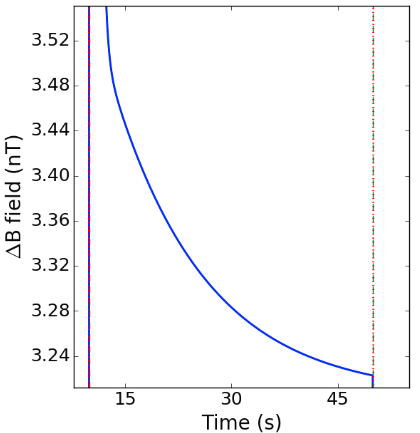
\includegraphics[width=\linewidth, height= 6.5 cm]{Images/i25_33_zoom.png}
        \caption{at $k_c^i$=0.25}
        \label{fig:i25zoom}
    \end{subfigure}%
    \begin{subfigure}{.5\linewidth}
        \centering
        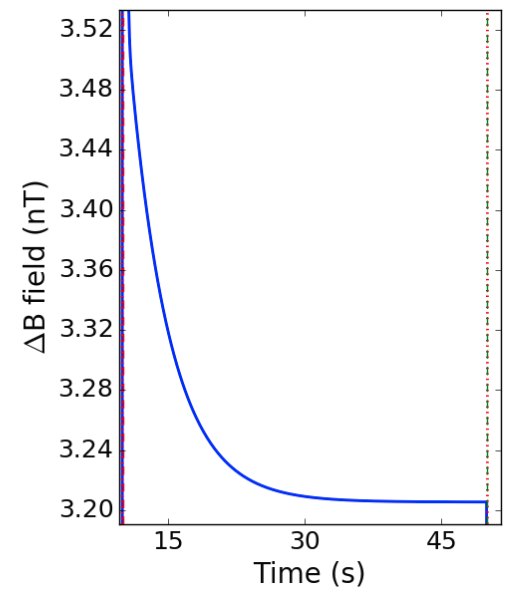
\includegraphics[width=\linewidth, height= 6.5 cm]{Images/i75_33_zoom.png}
        \caption{at $k_c^i$=0.75}
        \label{fig:i75zoom}
    \end{subfigure}\\[1ex]
    \begin{subfigure}{.5\linewidth}
        \centering
        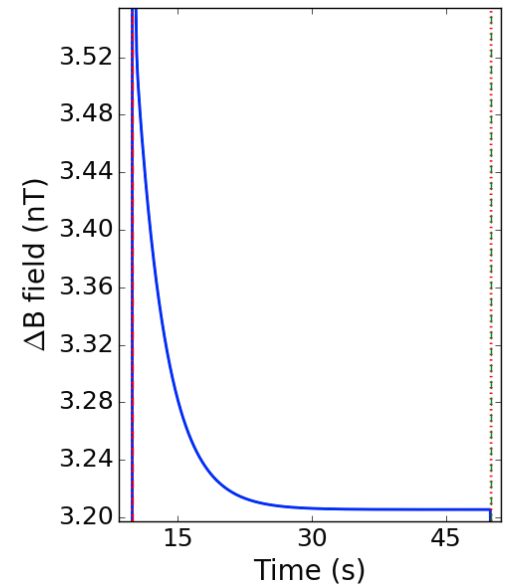
\includegraphics[width=\linewidth, height= 6.5 cm]{Images/i100_33_zoom.png}
        \caption{at $k_c^i$=1.0}
        \label{fig:i100zoom}
    \end{subfigure}%
        \begin{subfigure}{.5\linewidth}
        \centering
        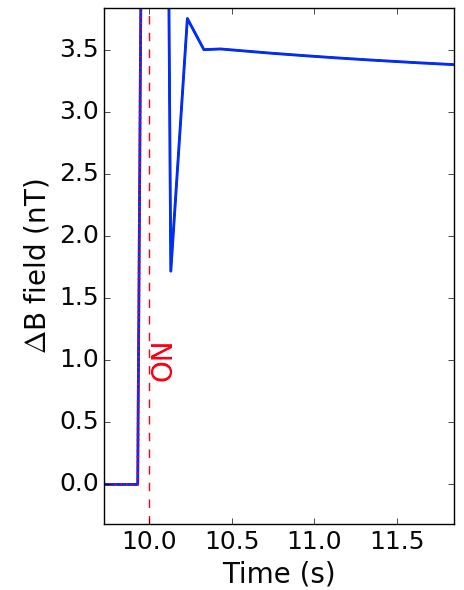
\includegraphics[width=\linewidth, height= 6.5 cm]{Images/i125_33_zoom.png}
        \caption{at $k_c^i$=1.25}
        \label{fig:i125zoom}
    \end{subfigure}

    \caption[short]{Zoomed in version of the drift $\Delta$B shown in right side of Fig.~\ref{fig:i_pi}\textcolor{blue}{(a)}, Fig.~\ref{fig:i_pi}\textcolor{blue}{(b)}, Fig.~\ref{fig:i_pi}\textcolor{blue}{(c)} and Fig.~\ref{fig:i_pi}\textcolor{blue}{(d)} respectively at sensor position '1x' for different values of $k_c^i$ with $k_c^p$ ( see Eq.~(\ref{eq:I}) ) being zero. The red vertical dashed line indicates the time of the perturbation coil being turned 'ON'. For position of coils and sensors see Fig.~\ref{fig: coil}.\label{fig:i_pi_zoom}}
\end{figure}

% \fig{Images/i_pi_zoom}{width = \textwidth,height =10cm}{Zoomed in version of the drift $\Delta$B shown in right side of Fig.~\ref{fig:i_pi}\textcolor{blue}{(a)}, Fig.~\ref{fig:i_pi}\textcolor{blue}{(b)}, Fig.~\ref{fig:i_pi}\textcolor{blue}{(c)} and Fig.~\ref{fig:i_pi}\textcolor{blue}{(d)} respectively at sensor position '1x' for different values of $k_c^i$ with $k_c^p$ ( see Eq.~(\ref{eq:I}) ) being zero. The red vertical dashed line indicates the time of the perturbation coil being turned 'ON'. For position of coils and sensors see Fig.~\ref{fig: coil}.\label{fig:i_pi_zoom}}


\FloatBarrier
The above results confirm that to get rid of the offsets that could not be reduce by the P term, an I term is a must. Next the effect of applying both of them after tuning (see Section~\ref{sec:tune}) will be discussed.
% \subsection{r vs. Condition No.}\label{sec:cond}
% Instead of going through all the steps that are discussed in Section~\ref{sec:inv}, the concept of condition number of a matrix can be used. The condition number of $\bm{M}$ can be determined from the diagonal matrix $\bm{\Sigma}$ as given in eq.\ref{eq:m} by -
%  \begin{equation}
%      cond(\bm{M})=\frac{max(\sigma_d)}{min(\sigma_d)}
%  \end{equation}
 

\subsubsection{Effect of changing PI term Combinely}
Finally, the Section~\ref{sec:pi_behave} will be ended here with the discussion of the effect of changing P and I term at a time which will complete the Eq.~(\ref{eq:I}).

Here, first the P and I term have been tuned following the discussion on Section~\ref{sec:tune} which has generated $k_c^p$=0.43 and $k_c^i$=0.52 . The results by applying $k_c^p$ and $k_c^i$ as those tuned values are shown in Fig.~\ref{fig:tuned_vs_i}\textcolor{blue}{(a)}. For simplicity instead of showing all the drift $\Delta$B for all the fluxgate sensors for the positions given in the horizonatal axis of Fig.~\ref{fig:m}, only '1x' is shown on the right of the figure. And same as earlier the currents  that are being sent to the coils ($C_x^\pm$, $C_y^\pm$ and $C_z^\pm$) shown on the left of the same figure. But, we couldn't determine the effect of having both of them at a time. So, keeping $k_c^i$ as 0.52 and excluding P term i.e. $k_c^p$=0.0 we run the same measurement again and the results are shwon in Fig.~\ref{fig:tuned_vs_i}\textcolor{blue}{(b)}. As as matter of surprise, there is hardly any difference between the results in Fig.~\ref{fig:tuned_vs_i}\textcolor{blue}{(a)} and Fig.~\ref{fig:tuned_vs_i}\textcolor{blue}{(b)}. Why is that so ? For the moment, the Fig.~\ref{fig:tuned_vs_i} suggests that may be we don't need P term at all or maybe we need different tuning methods. So, applying P and I term at a time raises question of the necessity of the P term or importance of the tuning method describe in Section~\ref{sec:tune}. Due to lack of time, we did not further go into other tuning methods. Rather we have tried to discover the differences in the work between Ref.~\cite{bea} and Ref.~\cite{rawlik}.
\doublefig{Images/p43i52_33}{width =\textwidth,height =8cm}{at $k_c^p$=0.43 and $k_c^i$=0.52. \label{fig:pi_tuned}}{Images/i52_33}{width = \textwidth,height =8cm}{at $k_c^p$=0.0 and $k_c^i$=0.52..\label{fig:i52}}{{Currents (left vertical axis) in all six coil sides ($C_x^\pm$, $C_y^\pm$ and $C_z^\pm$) with drift $\Delta$B (right vertical axis) at sensor position '1x' for combine different values of $k_c^i$ and $k_c^p$ ( see Eq.~(\ref{eq:I}) ). Blue color curve denotes the actual drift in signal at position '1x' found by Eq.~(\ref{eq:del_B}), while the red curve denotes the drift that would have been without the compensation. The 'ON' and 'OFF' vertical dashed lines indicate the time of the perturbation coil being turned 'ON' and 'OFF' respectively. For position of coils and fluxgate sensor see Fig.~\ref{fig: coil}.} \label{fig:tuned_vs_i}}{short}

\FloatBarrier
The above results give us confusion on the effectiveness of the P term and also the tuning method. Instead of looking more deep into tuning method, we moved our focused on the PI control equation explained by Ref.~\cite{bea} and Ref.~\cite{rawlik}.

\section{Style of PI (Old/New)}
We have talked about the tuning method in Section~\ref{sec:tune} and later in Section~\ref{sec:pi_behave} we have shown the the effect of the P and I term where the effectiveness of the P term and the tuning method arises. Those  were all based on the works from Ref.\cite{bea}. In early 2018, another author on his PhD thesis \cite{rawlik} claimed that there is no need of PI!! As we have done most of our work following the Ref.\cite{bea}, so we wanted to verify that the claim of no PI by Ref.\cite{rawlik} is actually true or not. So, this Section is all about comparing the work from two Ref.\cite{bea} and Ref.\cite{rawlik} and verify the claim. 

Here, the PI control algorithm as discussed by the Eq.~(\ref{eq:I}) which taken from Ref.~\cite{bea}) is termed as the 'Old PI' control. and no PI claim by Ref.~\cite{rawlik} is termed as 'New PI' control and the new current can be found by -
\begin{equation}\label{eq:I_raw}
    I^{n+1}= I^n+M^{-1} (B_{setpoint}-B_{measure}^n)=I^n+M^{-1} \Delta B^n
\end{equation}
or with a delay like -
\begin{equation}\label{eq:I_raw_delay}
    I^{n+1}= I^{n-2}+M^{-1} (B_{setpoint}-B_{measure}^n)=I^{n-2}+M^{-1} \Delta B^n
\end{equation}
But is it really possible ? 

To verify that we run the prototype two times. First time we set the value of $k_c^p$=0.0 and $k_c^i$=1.0 to find the new current by Eq.~(\ref{eq:I}) from 'Old PI' and another with $k_c^p$=1.0 and $k_c^i$=0.0 to find the new current determined by Eq.~(\ref{eq:I_raw}) of 'New PI'. The results from 'Old PI' are given in Fig.~\ref{fig:style_of_pi}\textcolor{blue}{(a)} and that of 'New PI' in Fig.~\ref{fig:style_of_pi}\textcolor{blue}{(b)}. For simplicity instead of showing all the drift $\Delta$B for all the fluxgate sensors for the positions given in the horizonatal axis of Fig.~\ref{fig:m}, only '1x' is shown on the right of the figures. And same as earlier the currents  that are being sent to the coils ($C_x^\pm$, $C_y^\pm$ and $C_z^\pm$) shown on the left of the same figures. It is seen that the results in both of the figures are same. That is P and I term of 'Old PI' has been transformed into I and P term of 'New PI' current equation.



\doublefig{Images/i100_old}{width =\textwidth, height= 6.5 cm}{at $k_c^p$=0.0 and $k_c^i$=1.0 for 'Old PI' \label{fig:i100_old}}{Images/p100_new}{width = \textwidth, height= 6.5 cm}{at $k_c^p$=1.0 and $k_c^i$=0.0 for 'New PI'\label{fig:p100_new}}{{Currents (left vertical axis) in all six coil sides ($C_x^\pm$, $C_y^\pm$ and $C_z^\pm$) with drift $\Delta$B (right vertical axis) at sensor position '1x' for combine different values of $k_c^i$ and $k_c^p$ by applying Eq.~(\ref{eq:I}) at (a) and Eq.~(\ref{eq:I_raw}) at (b) . Blue color curve denotes the actual drift in signal at position '1x' found by Eq.~(\ref{eq:del_B}), while the red curve denotes the drift that would have been without the compensation. The 'ON' and 'OFF' vertical dashed lines indicate the time of the perturbation coil being turned 'ON' and 'OFF' respectively. For position of coils and fluxgate sensor see Fig.~\ref{fig: coil}..} \label{fig:style_of_pi}}{short}


\FloatBarrier
But again is it really true about what we are claiming ?

To verify that the equation has been studied deeply. The mathematical equivalent of Eq.~(\ref{eq:I_raw}) is- 
\begin{equation}\label{eq:I_raw_eq}
    I^{n+1}= \sum_{i=0}^n M^{-1} (B_{setpoint}-B_{ambient}^i)
\end{equation}

The equivalency can be proved by mathematical induction. That is, for n$\geq$0, let $P_n$ be the following statement -
\begin{equation}\label{eq:I_raw_eq_both}
   I^n+M^{-1} (B_{setpoint}-B_{measure}^n)= \sum_{i=0}^n M^{-1} (B_{setpoint}-B_{ambient}^i)
\end{equation}

For n=0, the statement $P_0$ is-

\begin{align*}
    \begin{split}
      LHS &=I^0+M^{-1} (B_{setpoint}-B_{measure}^0) \\
        &=I^0+M^{-1} (B_{setpoint}-B_{ambient}^0 -M I^0) \\
        &=I^0+M^{-1} (B_{setpoint}-B_{ambient}^0) - MM^{-1} I^0) \\
        &=I^0+M^{-1} (B_{setpoint}-B_{ambient}^0) - I^0 \\
        &=M^{-1} (B_{setpoint}-B_{ambient}^0)
    \end{split}
    \\
    \begin{split}
      RHS &=M^{-1} (B_{setpoint}-B_{ambient}^0)\\
          &= LHS
    \end{split}
\end{align*}
$\therefore$ The Eq.~(\ref{eq:I_raw_eq_both}) is true for n=0.\newline
Suppose it is also true for k$\geq$0. That is, the following statement $P_k$ holds -
\begin{equation}\label{eq:I_raw_99}
   I^k+M^{-1} (B_{setpoint}-B_{measure}^k)= \sum_{i=0}^k M^{-1} (B_{setpoint}-B_{ambient}^i)
\end{equation}

It is to be showed that $P_{k+1}$ also holds, that is-

\begin{equation}\label{eq:I_raw_98}
   I^{k+1}+M^{-1} (B_{setpoint}-B_{measure}^{k+1})= \sum_{i=0}^{k+1} M^{-1} (B_{setpoint}-B_{ambient}^i)
\end{equation}
\begin{align*}
    \begin{split}
      LHS &=I^{k+1}+M^{-1} (B_{setpoint}-B_{measure}^{k+1}) \\
        &=I^{k+1}+M^{-1} (B_{setpoint}-B_{ambient}^{k+1} -M I^{k+1}) \\
        &=I^{k+1}+M^{-1} (B_{setpoint}-B_{ambient}^{k+1}) - MM^{-1} I^{k+1}) \\
        &=I^{k+1}+M^{-1} (B_{setpoint}-B_{ambient}^0) - I^{k+1} \\
        &=M^{-1} (B_{setpoint}-B_{ambient}^{k+1})
    \end{split}
    \\
    \begin{split}
      RHS &=M^{-1} (B_{setpoint}-B_{ambient}^{k+1})\\
          &= LHS
    \end{split}
\end{align*}
$\therefore \: P_{k+1}$ also holds which validates the Eq.~(\ref{eq:I_raw_eq_both}) by the principle of mathematical induction. \newline
Now, the Eq.~(\ref{eq:I_raw_eq}) is equivalent to the implementation of PI -
\begin{equation}\label{eq:I_raw_pi}
    I^{n+1}= k_p E^n+ k_i \sum_{i=0}^n E^i \Delta t
\end{equation}
with $k_p=0$ and $k_i$ set to a particular value. Here, the error is , $E^i=M^{-1} (B_{setpoint}-B_{ambient}^i)$. So, the Eq.~(\ref{eq:I_raw}) is a PI with a particular tuning and termed as 'New PI' control. Similarly, the delay showed in Eq.~(\ref{eq:I_raw_delay}) is another form of tuning.

So the above discussion verifies that 'Old PI' and 'New PI' are just two different form of tuning based on the control algorithm. We can also clear our previous questions about the effectiveness of the P term and the tuning method discussed in Section~\ref{sec:pi_behave} that instead of the tuning method discussed in Section~\ref{sec:tune}, we are using different from of tuning with changing the value of $k_c^i$ keeping $k_c^p$=0. In upcoming Section we then studied the effect of  matrix condition number in P and I term. and propose a new method to find regularization parameter using matrix condition number. 



\section{New Studies on Regularization Parameter}\label{sec:new_study_r}
In Section~\ref{sec:inv} we have introduced the regularization parameter 'r' and then discussed a simulation model in Section~\ref{sec:mont} which later has been justified by comparing with experimental setup in Section~\ref{fig:mont_comp}. We have also talked about the PI behaviour in Section~\ref{sec:pi_behave}. Here, we will first show the effect of matrix condition number on PI behaviour and then propose a new method to find 'r' based on condition number of matrix. 

So, first the importance of matrix condition number on PI will be discussed.

\subsection{Importance of Matrix Condition Number on PI}\label{sec:pi_behave_m}
Matrix Condition number ( see Eq.~(\ref{eq:cond} ) have been introduced in Section.~\ref{sec:m} while discussing the inversion of the matrix $\bm{M}$ . An ill-conditioned matrix has large condition number and a matrix with small condition number is said to be well-conditioned. Here, the effect of matrix condition number on PI will be discussed in terms of a very large condition number that is 129.
 
\subsubsection{Condition Number Effect on changing only P term}
Here, the effect of changing proportional gain term (P) or $k_c^p$ of Eq.~(\ref{eq:I}) will be discussed for a matrix condition number of 129 which is very ill-conditioned compared to 33 discussed in Section~\ref{sec:pi_behave}.

P term is proportionally multiplying the error (the difference between setpoint and actual measurement) with a constant gain and discussed more in Section~\ref{sec:pi_behave}.


\begin{figure}[!htb]
    \begin{subfigure}{.5\linewidth}
        \centering
        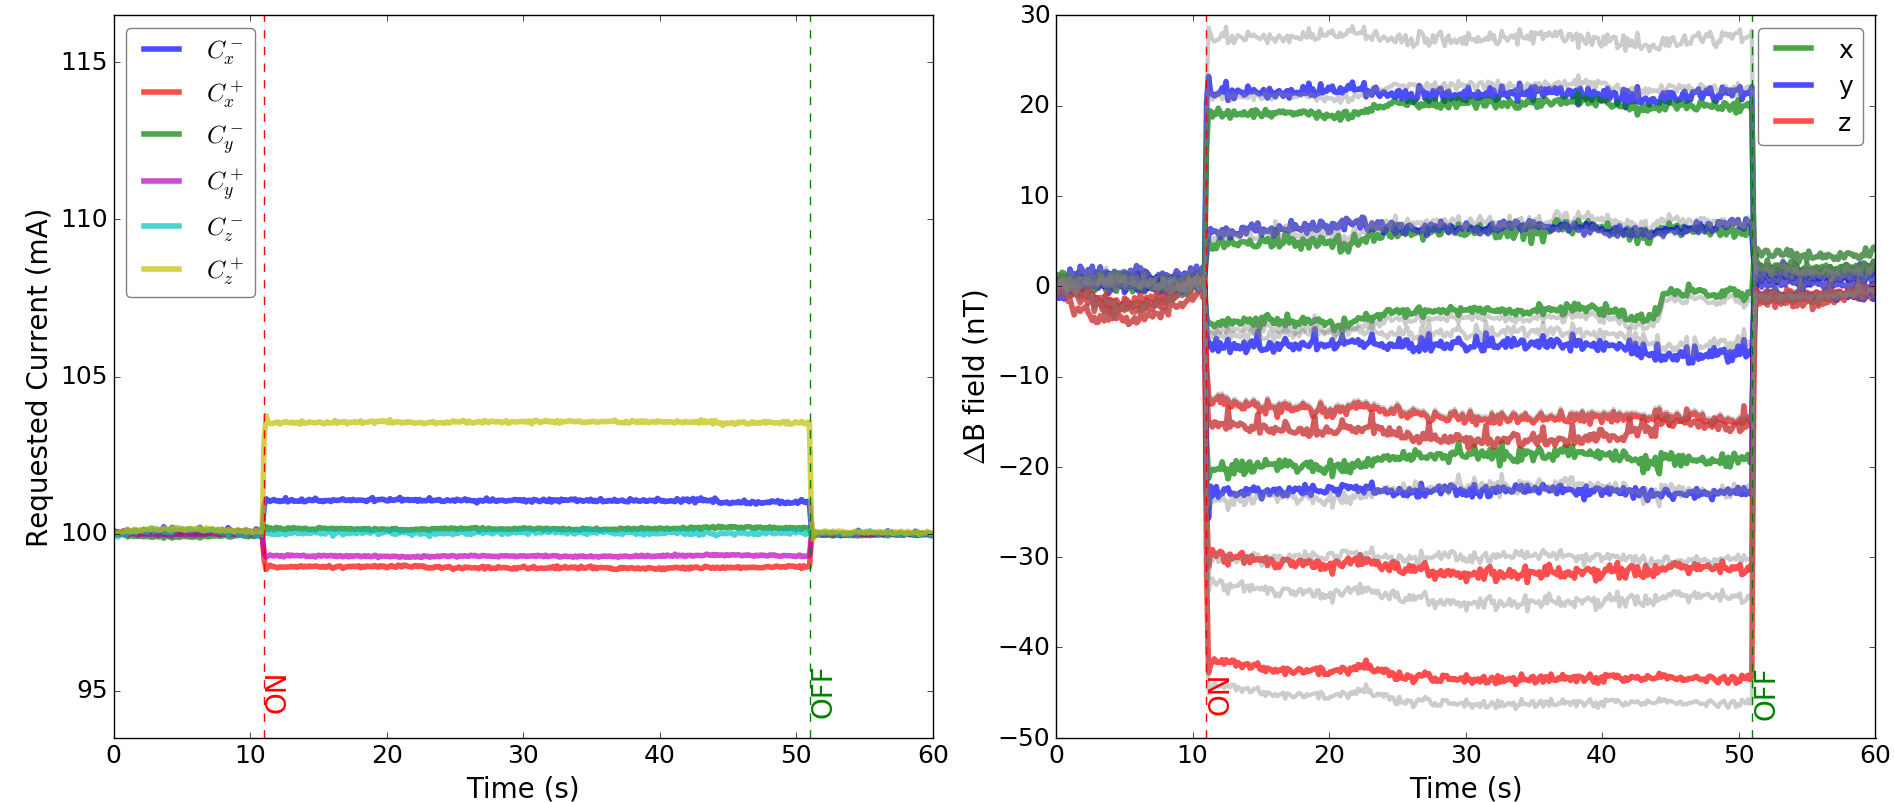
\includegraphics[width=\linewidth, height= 6.5 cm]{Images/p25}
        \caption{at $k_c^p$=0.25}
        \label{fig:p25m}
    \end{subfigure}%
    \begin{subfigure}{.5\linewidth}
        \centering
        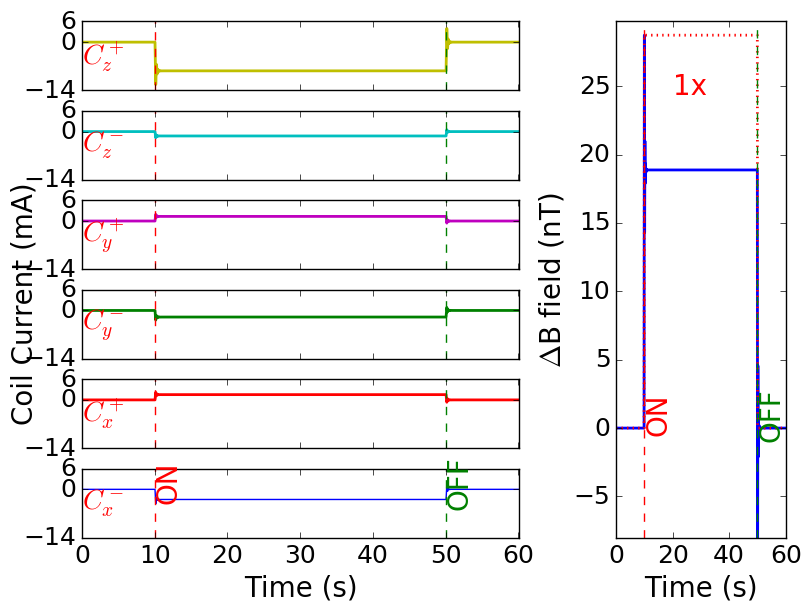
\includegraphics[width=\linewidth, height= 6.5 cm]{Images/p50}
        \caption{at $k_c^p$=0.50}
        \label{fig:p50m}
    \end{subfigure}\\[1ex]
    \begin{subfigure}{.5\linewidth}
        \centering
        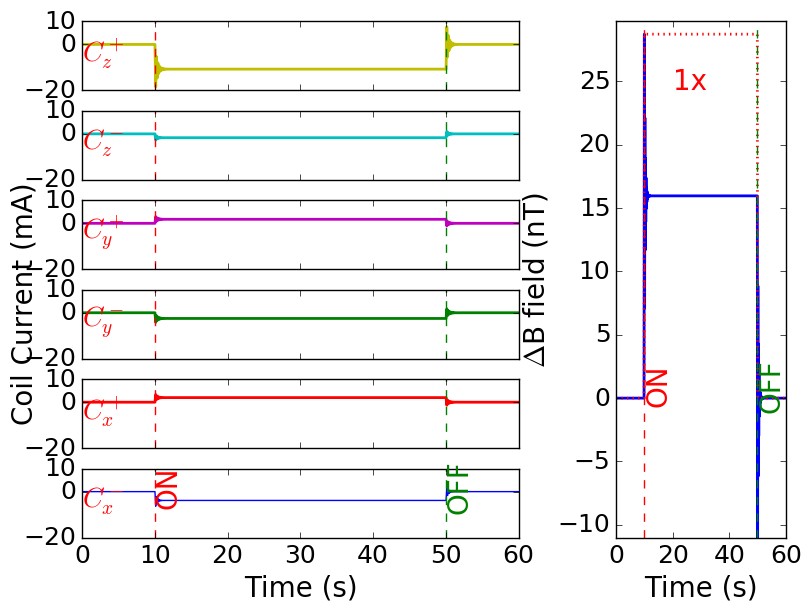
\includegraphics[width=\linewidth, height= 6.5 cm]{Images/p75}
        \caption{at $k_c^p$=0.75}
        \label{fig:p75m}
    \end{subfigure}%
        \begin{subfigure}{.5\linewidth}
        \centering
        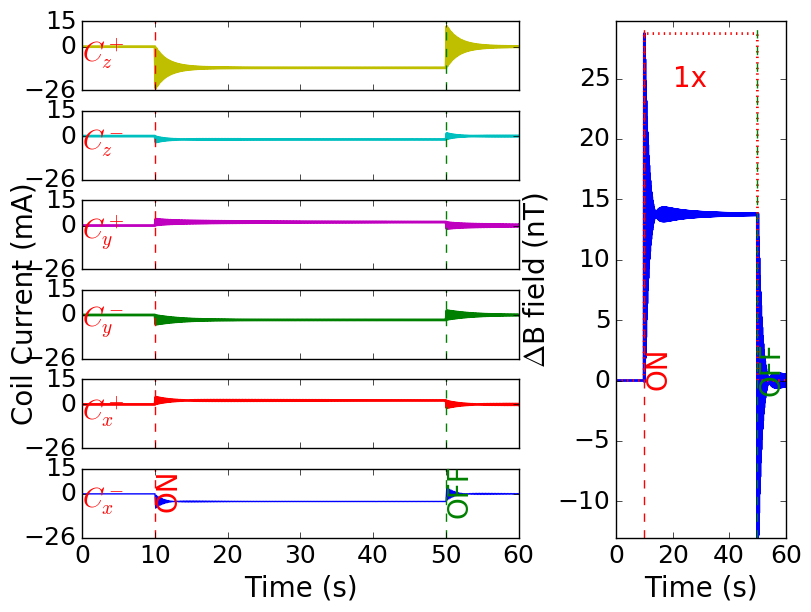
\includegraphics[width=\linewidth, height= 6.5 cm]{Images/p100}
        \caption{at $k_c^p$=1.0}
        \label{fig:p100m}
    \end{subfigure}

    \caption[short]{Currents (left vertical axis) in all six coil sides ($C_x^\pm$, $C_y^\pm$ and $C_z^\pm$) with drift $\Delta$B (right vertical axis) at sensor position '1x' for different values of $k_c^p$ with $k_c^i$ in Eq.~(\ref{eq:I}) being zero. Blue color curve denotes the actual drift in signal at position '1x' found by Eq.~(\ref{eq:del_B}) while the red curve denotes the drift that would have been without the compensation. The 'ON' and 'OFF' vertical dashed lines indicate the time of the perturbation coil being turned 'ON' and 'OFF' respectively. For position of coils and sensors see Fig.~\ref{fig: coil}. }
    \label{fig:p_pi_m}
\end{figure}

The effect of changing $k_c^p$ has been shown in Fig.~\ref{fig:p_pi_m} where the currents (left) that are being sent to the coils ($C_x^\pm$, $C_y^\pm$ and $C_z^\pm$) for drift $\Delta$B found by Eq.~(\ref{eq:del_B}) in sensor position '1x'.  It is seen that $\Delta$B=23 nT, 18.5 nT and 16.5 nT for $k_c^p$ = 0.25, 0.5 and 0.75 respectively (see Fig.~\ref{fig:p_pi_m}\textcolor{blue}{(a)}, Fig.~\ref{fig:p_pi_m}\textcolor{blue}{(b)}, Fig.~\ref{fig:p_pi_m}\textcolor{blue}{(c)}). That is, with the increase of $k_c^p$, $\Delta$B magnetic field decreases. But, it has a limit after which with the increase of $k_c^p$, the systems becomes unstable and starts oscillating which can be seen from Fig.~\ref{fig:p_pi_m}\textcolor{blue}{(d)}) where the currents (left) are oscillating and the drift itself also at $\Delta$B=14.5 nT (right). So, the error is reduced maximum by (29.5-14.5)/29.5 * 100$\%\approx$51$\%$ from the initial drift of $\Delta$B=29.5 nT denoted by the red curve at position '1x'. 

\FloatBarrier
The above results confirm that matrix condition number has minimal effect on P term by comparing the effect shown in Section~\ref{sec:pi_behave}. Next, we will discuss about the effect on only I term.

\subsubsection{Condition Number Effect on Changing only I term}
Here, the effect matrix condition number effect on changing integral reset term (I) or $k_c^i$ of Eq.~(\ref{eq:I}) will be discussed.

The error (the difference between setpoint and actual measurement) is accumulated for the length of measurements and I term is multiplying that accumulated error  with a constant gain as discussed in Section~\ref{sec:pi_behave}.




As like the effect on P, the effect of changing $k_c^i$ has been shown in Fig.~\ref{fig:i_pi_m} where the currents (left) that are being sent to the coils ($C_x^\pm$, $C_y^\pm$ and $C_z^\pm$) for drift $\Delta$B found by Eq.~(\ref{eq:del_B}) in sensor position '1x' for $k_c^i$=0.25, 0.5, 0.75 and 1.0.  It is seen from Fig.~\ref{fig:i_pi_m}\textcolor{blue}{(a)}, Fig.~\ref{fig:i_pi_m}\textcolor{blue}{(b)}, Fig.~\ref{fig:i_pi_m}\textcolor{blue}{(c)} and Fig.~\ref{fig:i_pi_m}\textcolor{blue}{(d)}). which are correspond to $k_c^i$ = 0.25, 0.75, 1.0 and 1.25 respectively that the error level (right) is $\sim$3.5 nT in every case, the coil currents(left) never settle in any of them which is not he case for low matrix condition number as seen from Fig.~\ref{fig:i_pi}\textcolor{blue}{(a)}, Fig.~\ref{fig:i_pi}\textcolor{blue}{(b)}, Fig.~\ref{fig:i_pi}\textcolor{blue}{(c)} and Fig.~\ref{fig:i_pi}\textcolor{blue}{(d)}) where the condition number is 33 compared to 129 here.

\begin{figure}[!htb]
    \begin{subfigure}{.5\linewidth}
        \centering
        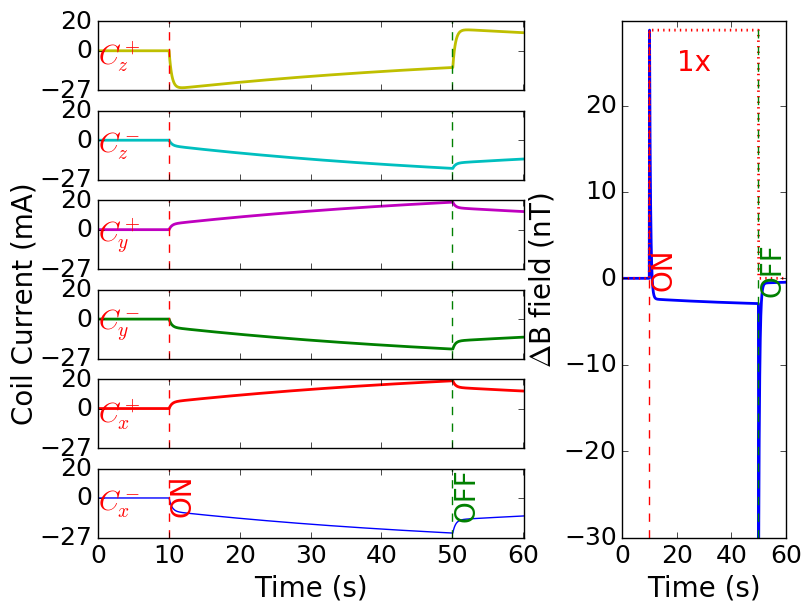
\includegraphics[width=\linewidth, height= 6.5 cm]{Images/i25}
        \caption{at $k_c^i$=0.25}
        \label{fig:i25m}
    \end{subfigure}%
    \begin{subfigure}{.5\linewidth}
        \centering
        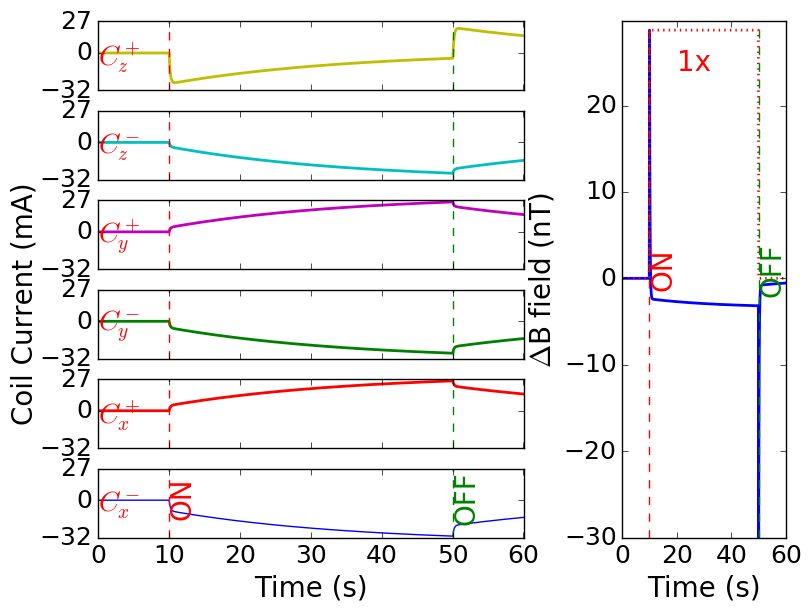
\includegraphics[width=\linewidth, height= 6.5 cm]{Images/i50}
        \caption{at $k_c^i$=0.5}
        \label{fig:i50m}
    \end{subfigure}\\[1ex]
    \begin{subfigure}{.5\linewidth}
        \centering
        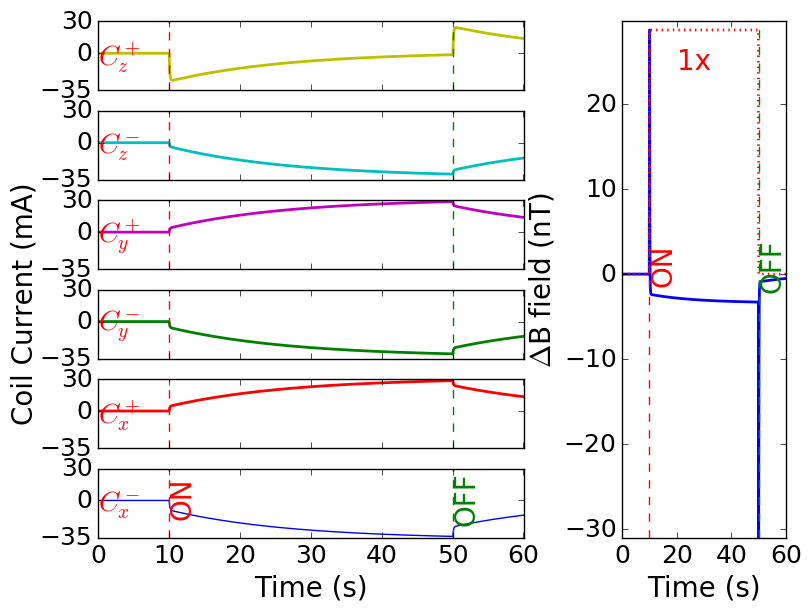
\includegraphics[width=\linewidth, height= 6.5 cm]{Images/i75}
        \caption{at $k_c^i$=0.75}
        \label{fig:i75m}
    \end{subfigure}%
        \begin{subfigure}{.5\linewidth}
        \centering
        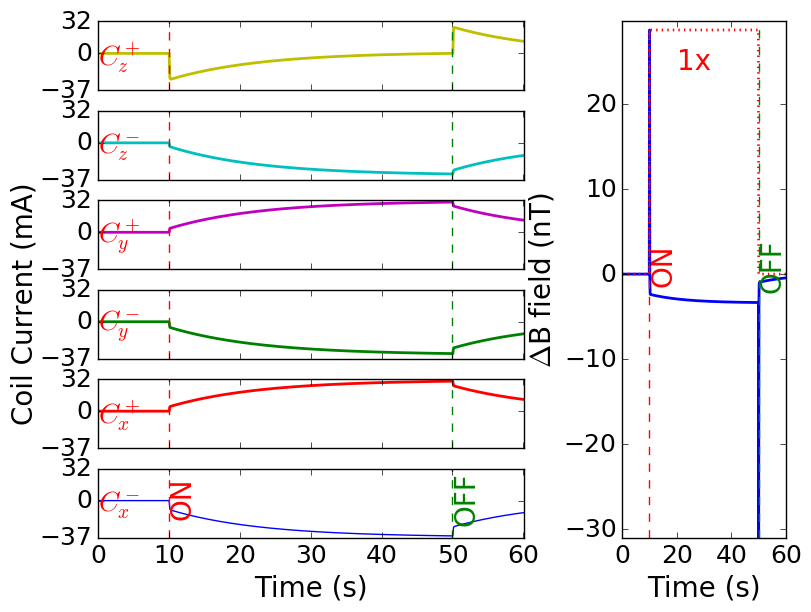
\includegraphics[width=\linewidth, height= 6.5 cm]{Images/i100}
        \caption{at $k_c^i$=1.0}
        \label{fig:i100m}
    \end{subfigure}

    \caption[short]{Currents (left vertical axis) in all six coil sides ($C_x^\pm$, $C_y^\pm$ and $C_z^\pm$) with drift $\Delta$B (right vertical axis) at sensor position '1x' for different values of $k_c^i$ with $k_c^p$ ( see Eq.~(\ref{eq:I}) ) being zero. Blue color curve denotes the actual drift in signal at position '1x' found by Eq.~(\ref{eq:del_B}) while the red curve denotes the drift that would have been without the compensation. The 'ON' and 'OFF' vertical dashed lines indicate the time of the perturbation coil being turned 'ON' and 'OFF' respectively. For position of coils and sensors see Fig.~\ref{fig: coil}.}
    \label{fig:i_pi_m}
\end{figure}



% \fig{Images/i_pi_zoom}{width = \textwidth,height =10cm}{Zoomed in version of the drift $\Delta$B shown in right side of Fig.~\ref{fig:i_pi}\textcolor{blue}{(a)}, Fig.~\ref{fig:i_pi}\textcolor{blue}{(b)}, Fig.~\ref{fig:i_pi}\textcolor{blue}{(c)} and Fig.~\ref{fig:i_pi}\textcolor{blue}{(d)} respectively at sensor position '1x' for different values of $k_c^i$ with $k_c^p$ ( see Eq.~(\ref{eq:I}) ) being zero. The red vertical dashed line indicates the time of the perturbation coil being turned 'ON'. For position of coils and sensors see Fig.~\ref{fig: coil}.\label{fig:i_pi_zoom}}


\FloatBarrier
The above results confirm the currents in the coils never settles in if there is a ill-conditioned matrix present.. Next the condition number effect on both both of them after tuning (see Section~\ref{sec:tune}) will be discussed and may be the currents settle there!!


% \subsection{r vs. Condition No.}\label{sec:cond}
% Instead of going through all the steps that are discussed in Section~\ref{sec:inv}, the concept of condition number of a matrix can be used. The condition number of $\bm{M}$ can be determined from the diagonal matrix $\bm{\Sigma}$ as given in eq.\ref{eq:m} by -
%  \begin{equation}
%      cond(\bm{M})=\frac{max(\sigma_d)}{min(\sigma_d)}
%  \end{equation}
 

\subsubsection{Condition Number Effect of changing PI term Combinely}
Finally, the Section~\ref{sec:pi_behave_m} will be ended here with the discussion of the condition number effect on changing P and I term at a time which will complete the Eq.~(\ref{eq:I}).

Here, first the P and I term have been tuned following the discussion on Section~\ref{sec:tune} which has generated $k_c^p$=0.43 and $k_c^i$=0.52 . The results by applying $k_c^p$ and $k_c^i$ as those tuned values are shown in Fig.~\ref{fig:tuned_vs_i}\textcolor{blue}{(a)}. For simplicity instead of showing all the drift $\Delta$B for all the fluxgate sensors for the positions given in the horizonatal axis of Fig.~\ref{fig:m}, only '1x' is shown on the right of the figure. And same as earlier the currents  that are being sent to the coils ($C_x^\pm$, $C_y^\pm$ and $C_z^\pm$) shown on the left of the same figure. But, we couldn't determine the effect of having both of them at a time. So, keeping $k_c^i$ as 0.52 and excluding P term i.e. $k_c^p$=0.0 we run the same measurement again and the results are shwon in Fig.~\ref{fig:tuned_vs_i_m}\textcolor{blue}{(b)}. The results of Fig.~\ref{fig:tuned_vs_i_m}\textcolor{blue}{(a)} are similar to that of Fig.~\ref{fig:tuned_vs_i_m}\textcolor{blue}{(b)} which is also true for low condition number as discussed in Section~\ref{sec:pi_behave}. 

\doublefig{Images/p43i52}{width =\textwidth,height =8cm}{at $k_c^p$=0.43 and $k_c^i$=0.52. \label{fig:pi_tuned_m}}{Images/i52}{width = \textwidth,height =8cm}{at $k_c^p$=0.0 and $k_c^i$=0.52..\label{fig:i52m}}{{Currents (left vertical axis) in all six coil sides ($C_x^\pm$, $C_y^\pm$ and $C_z^\pm$) with drift $\Delta$B (right vertical axis) at sensor position '1x' for combine different values of $k_c^i$ and $k_c^p$ ( see Eq.~(\ref{eq:I}) ). Blue color curve denotes the actual drift in signal at position '1x' found by Eq.~(\ref{eq:del_B}), while the red curve denotes the drift that would have been without the compensation. The 'ON' and 'OFF' vertical dashed lines indicate the time of the perturbation coil being turned 'ON' and 'OFF' respectively. For position of coils and fluxgate sensor see Fig.~\ref{fig: coil}.} \label{fig:tuned_vs_i_m}}{short}

\FloatBarrier
The above results rather confirm that matrix condition number does not bring any change while using P and  term at a time. But it has got huge impact on I term for which the coil current never settles in case of ill conditioned matrix. Next we will try to improve the current settling problem by changing the regularization parameter.

\subsection{Effect of 'r' on PI Tuning}\label{sec:r_pi}

The discussion on Section~\ref{sec:pi_behave_m} suggests that I term is necessary for fast system response due to any drift in the magnetic signal as it takes care of the offset problems which is unsolvable by using only P term. But, in doing so, it also creates problems in terms of the coil currents which never settle in for the duration of the perturbation in case of ill-conditioned matrix. The tuning method described in Section~\ref{sec:tune} should have take care of this but we have realized that having tuned P and I has similar effect like having only I term. So, tuning method doesn't give us the solution. Rather looking for different tuning method , we have focused on the effect of 'r' on PI tuning. This Section will discuss that effect with possible outcome.

The experimental setup is same as discussed in Section~\ref{sec:pi_behave_m}. But in this case we have chosen $k_c^p$=0 and $k_c^i$=0.52. Among those $k_c^i$=0.52 has been found due to PI tuning (see Section~\ref{sec:tune}) and instead of choosing  $k_c^p$=0.43 we have made this zero as from the earlier discussion we saw that it barely has any effect while we use the I term. So, these values of $k_c^p$ and $k_c^i$ will be applied on Eq.~\ref{eq:I} to find the currents to be sent to the coils ($C_x^\pm$, $C_y^\pm$ and $C_z^\pm$) for drift $\Delta$B found by Eq.~(\ref{eq:del_B}) in the sensor positions given in the horizontal axis of Fig.~\ref{fig:m}. So, keeping those fixed, we will try to change the value of 'r' which will modify the Eq.~(\ref{eq:minvR}) for each change of 'r' value.

The effect of changing 'r' with $k_c^p$=0 and $k_c^i$=0.52 has been shown in Fig.~\ref{fig:r_pi} where the currents (left) that are being sent to the coils ($C_x^\pm$, $C_y^\pm$ and $C_z^\pm$) for drift $\Delta$B found by Eq.~(\ref{eq:del_B}) in sensor position '1x'.  It is seen from Fig.~\ref{fig:r_pi}\textcolor{blue}{(a)}, Fig.~\ref{fig:r_pi}\textcolor{blue}{(b)}, Fig.~\ref{fig:r_pi}\textcolor{blue}{(c)} and Fig.~\ref{fig:r_pi}\textcolor{blue}{(d)} which are correspond to 'r' = 2.0, 2.4, 2.8 and 3.2 respectively that the changing 'r' has significant effect on the coil current graph and barely any effect on the system response time for reducing the drift in the signal. That is at 'r'=2.0, the coil current graph has the fastest settling time where the current settles within 3 s after the perturbation has been applied. At 'r'=2.4, it takes 10s for the coil currents to settle in. But at 'r'=2.8, it seems like the coil current never settles in which is again improved at 'r'=3.2. Note that the here seriously ill conditioned matrix with condtion number 129 has been used and optimized 'r' found by the simulation model is $\sim$2.9 which tells us that the coil settling of the current graph seems to have issue with the that optimized 'r for ill-conditioned matrix. So, instead of taking the optimized 'r' that has been found by the simulation model we may have to choose the lower value of 'r'. 

\begin{figure}[!htb]
    \begin{subfigure}{.5\linewidth}
        \centering
        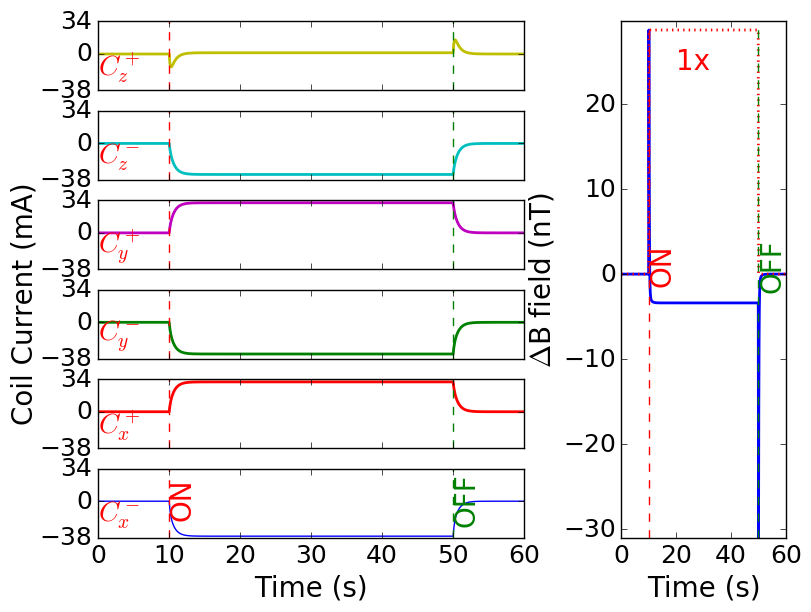
\includegraphics[width=\linewidth, height= 6.5 cm]{Images/r20}
        \caption{at r=2.0}
        \label{fig:r20}
    \end{subfigure}%
    \begin{subfigure}{.5\linewidth}
        \centering
        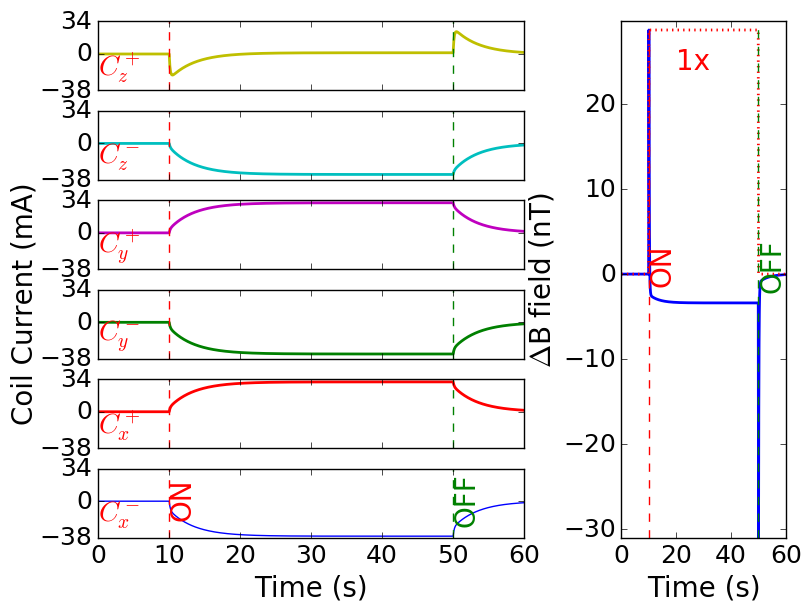
\includegraphics[width=\linewidth, height= 6.5 cm]{Images/r24}
        \caption{at r=2.4}
        \label{fig:r24}
    \end{subfigure}\\[1ex]
    \begin{subfigure}{.5\linewidth}
        \centering
        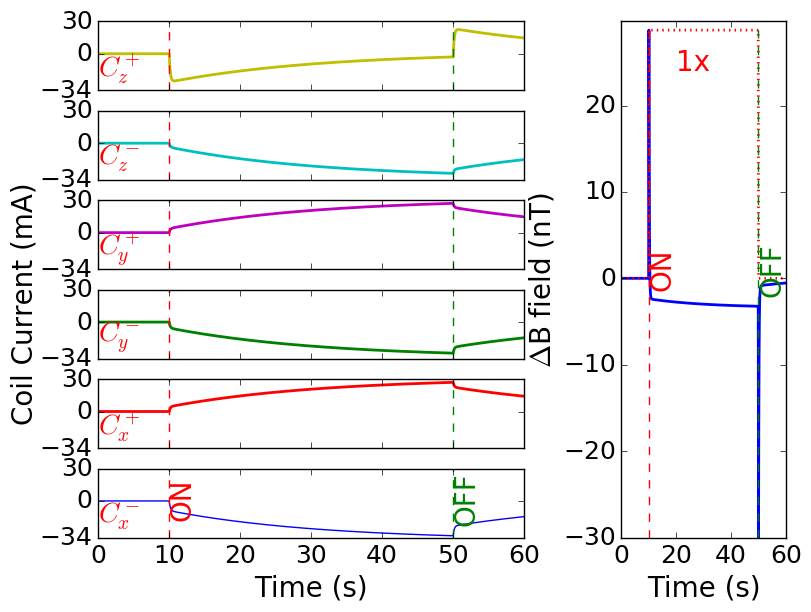
\includegraphics[width=\linewidth, height= 6.5 cm]{Images/r28}
        \caption{at r=2.8}
        \label{fig:r28}
    \end{subfigure}%
        \begin{subfigure}{.5\linewidth}
        \centering
        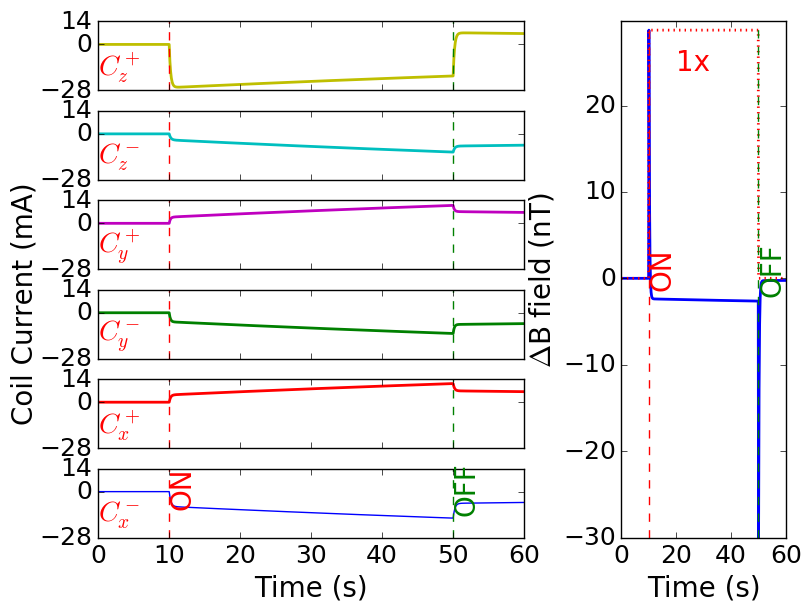
\includegraphics[width=\linewidth, height= 6.5 cm]{Images/r32}
        \caption{at r=3.2}
        \label{fig:r32}
    \end{subfigure}


    \caption[short]{Currents (left vertical axis) in all six coil sides ($C_x^\pm$, $C_y^\pm$ and $C_z^\pm$) with drift $\Delta$B (right vertical axis) at sensor position '1x' for combine different values of $k_c^i$ and $k_c^p$ ( see Eq.~(\ref{eq:I}) ). Blue color curve denotes the actual drift in signal at position '1x' found by Eq.~(\ref{eq:del_B}), while the red curve denotes the drift that would have been without the compensation. The 'ON' and 'OFF' vertical dashed lines indicate the time of the perturbation coil being turned 'ON' and 'OFF' respectively. For position of coils and fluxgate sensor see Fig.~\ref{fig: coil}.}
    \label{fig:r_pi}
\end{figure}

\FloatBarrier
Now the question arises about what if 'r' value is chosen more than the optimized 'r'. For answering that question, we have also studied the effect for more values of 'r' with same setup which are shown in Fig.~\ref{fig:r_pi_more}. It is seen from Fig.~\ref{fig:r_pi_more}\textcolor{blue}{(a)}, Fig.~\ref{fig:r_pi_more}\textcolor{blue}{(b)}, Fig.~\ref{fig:r_pi_more}\textcolor{blue}{(c)} and Fig.~\ref{fig:r_pi_more}\textcolor{blue}{(d)} which are correspond to 'r' = 3.5, 3.6, 3.7 and 3.9 respectively that the coil current graph seems to be settle in for larger value of 'r' before it starts showing less responsive for example at 'r'=3.9.   

\begin{figure}[!htb]
    \begin{subfigure}{.5\linewidth}
        \centering
        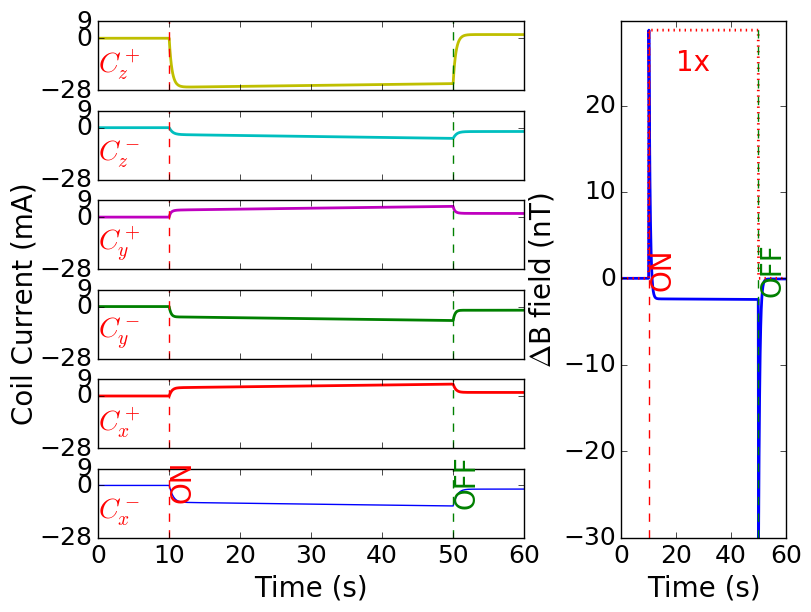
\includegraphics[width=\linewidth, height= 6.5 cm]{Images/r35}
        \caption{at r=3.5}
        \label{fig:r35}
    \end{subfigure}%
    \begin{subfigure}{.5\linewidth}
        \centering
        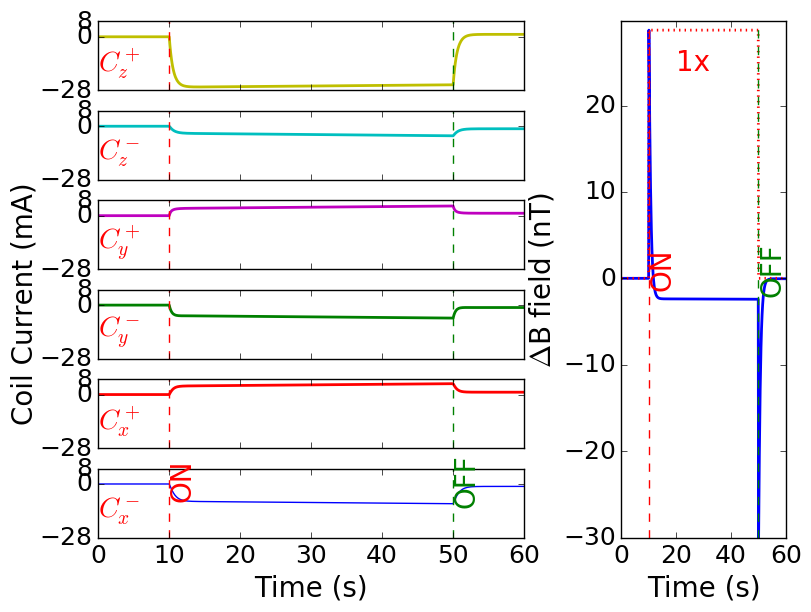
\includegraphics[width=\linewidth, height= 6.5 cm]{Images/r36}
        \caption{at r=3.6}
        \label{fig:r36}
    \end{subfigure}\\[1ex]
    \begin{subfigure}{.5\linewidth}
        \centering
        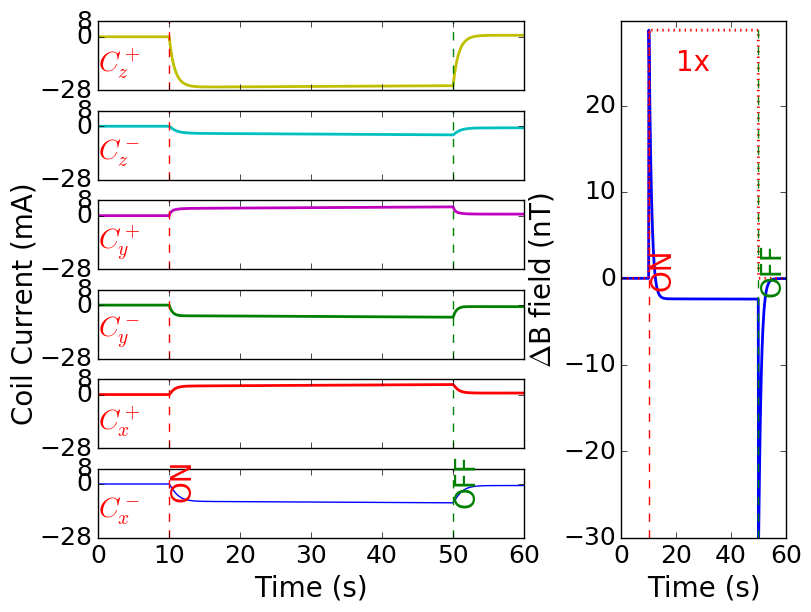
\includegraphics[width=\linewidth, height= 6.5 cm]{Images/r37}
        \caption{at r=3.7}
        \label{fig:r37}
    \end{subfigure}%
        \begin{subfigure}{.5\linewidth}
        \centering
        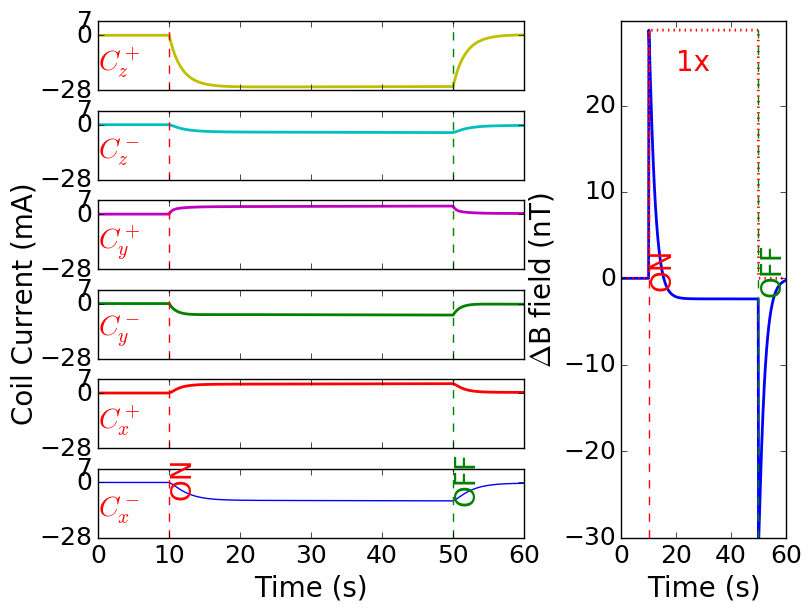
\includegraphics[width=\linewidth, height= 6.5 cm]{Images/r39}
        \caption{at r=3.9}
        \label{fig:r39}
    \end{subfigure}


    \caption[short]{Currents (left vertical axis) in all six coil sides ($C_x^\pm$, $C_y^\pm$ and $C_z^\pm$) with drift $\Delta$B (right vertical axis) at sensor position '1x' for combine different values of $k_c^i$ and $k_c^p$ ( see Eq.~(\ref{eq:I}) ). Blue color curve denotes the actual drift in signal at position '1x' found by Eq.~(\ref{eq:del_B}), while the red curve denotes the drift that would have been without the compensation. The 'ON' and 'OFF' vertical dashed lines indicate the time of the perturbation coil being turned 'ON' and 'OFF' respectively. For position of coils and fluxgate sensor see Fig.~\ref{fig: coil}.}
    \label{fig:r_pi_more}
\end{figure}

\FloatBarrier

The above results confirm that for a matrix with large condition number, the value of 'r' has to be tuned alongside the PI tuning. Next we will talk about a new method to find 'r'.

\subsection{Regularization by Matrix Condition Number Method  }\label{sec:cond}
We have talked about the importance of matrix condition number on PI tuning. Matrix Condition number ( see Eq.~(\ref{eq:cond} ) and regularization parameter 'r' ( see Eq.~(\ref{eq:minvR} ) have been introduced in Section.~\ref{sec:m} while discussing the inversion of the matrix $\bm{M}$ . Moreover, in Section~\ref{sec:mont}, a method of regularization by random fluctuation has been discussed. Here, we will propose another method of regularization using the concept of matrix condition number.
 
 Recall from Section~\ref{sec:inv}, regularization is needed in the first place while inverse of the matrix $\bm{M}$ because $\bm{M}$ itself is ill-conditioned matrix. That means the $\bm{M}$ has a large condition number which while inverse would produce large currents in some ill-positioned places that will make the system unstable. So, it is required to have a well-conditioned  $\bm{M^{-1}}$ which implies that the condition number of $\bm{M^{-1}}$ should be small and that's what regularization has been doing. So, we introduce Eq.~\ref{eq:minvR} with various values of 'r' and each time the condition number of $\bm{M^{-1}}$ is stored. Then the optimized 'r'  has been determined by selecting the 'r' for which the condition number of $\bm{M^{-1}}$ is the minimum.
 
 The condition number of $\bm{M^{-1}}$ for different values of 'r' has been shown in Fig.~\ref{fig:cond}. It is seen that for 'r'=0, the condition number of $\bm{M^{-1}}$=$\sim$40 that is same as the condition number of $\bm{M}$ itself. So, without regularization that is the condition number of pseudo-inverse of $\bm{M}$ would also give =$\sim$40. In regularization method, several 'r' is tried ( see Eq.~(\ref{eq:minvR}) ) and each time the condition number has been stored which are shown in the vertical axis. The red diamond symbol indicates that for 'r'=2.94, the condition number of $\bm{M^{-1}}$ is minimum and that is 3.1. That by using 'r'=2.94 in Eq.~(\ref{eq:minvR}), the condition number decrease from 40 to 3.1 which is 40/3.1$\approx$13 times of decrements. The Fig.~\ref{fig:I-fluc} shows that the 'r'=2.87 compared to 'r'=2.94 that we found here. So, both method shows comparable result. This method will always produce fixed optimized 'r' for a particular  $\bm{M}$ but the method by random fluctuation (see Section~\ref{sec:mont}) will produce different optimize 'r' for different run as it because depends on the random field.

 
\fig{Images/6c_Mcond}{width = \textwidth,height =10cm}{Condition Number of $\bm{M^{-1}}$ (vertical axis) for different values of 'r. The matrix is same as described by the Fig.~\ref{fig:m}.  \label{fig:cond}}{short}

\FloatBarrier

In the above, different method to find optimize 'r' has been discussed which is a good alternative to the one explained in Section~\ref{sec:mont} and the results are similar. In upcoming Section we will discuss fluxgate placement and impact of different shields.


% \subsubsection{Optimized r  Revisited Based on Current Response Time}\label{sec:r_currentResponse}
% It was found that there is very slow coil current rise time while applying perturbation. To get rid of that problem, first and foremost, the fastest sampling frequency (see section [\ref{sec:filter}, \ref{sec:freq}]) is needed. Then, the next step of the problem can be solved via two ways with individual having own limitations. First way is tuning the value of P and I term of PI loop as explained in Eq.~(\ref{eq:I} and Section~\ref{sec:tune}. But with increasing the value of P, the current start oscillating after certain values as shown by the top and middle current graph on Fig.~\ref{fig:crnt} which is a problem. 

% \fig{Images/crnt}{width = \textwidth}{Coil current in one of the coil side for optimized r=2.8 with P=0 and I=1.0 (top) and with P=0 and I=1.5 (middle) and for best r considering noise with P=0 and I=1.0 (bottom). \label{fig:crnt}}



% The alternative way is to change the value of optimized r (see section [\ref{sec:mont}, \ref{sec:cond}]) which in turns increase noise in the prototype. But with inclusion of some current fluctuations, it was found that the coil current response time was increased heavily  as shown by the bottom current graph in Fig.~\ref{fig:crnt}. Now, the best compromised value of r was chosen by observing the 'rise time vs r' and 'fluctuations vs r' as shown in Fig.~\ref{fig:riseT}.



%  \doublefig{Images/riseT}{width =\textwidth, height= 8 cm}{Rise Time vs r \label{fig:rise}}{Images/fluc}{width = \textwidth, height= 8 cm}{Fluctuations\label{fig:fluc}}{{(a) shows the Rise Time vs r (b) shows the Fluctuations } \label{fig:riseT}}
% % \fig{Images/bt}{width = \textwidth}{Magnetic Field Compensation \label{fig:bt}}






\section{Fluxgate Placements and Impact of Shields}


In earlier section we have shown results using 12 fluxgate sensors placed at positions as given in horizonatal axis of Fig.~\ref{fig:m} and there exact positions are described by the Fig.~\ref{fig: coil}. We were facing serious problem with coil current not being settle properly although the field seems to be compensated on time. So, we have tried different posoitions mainly in corners and center of each of the coil faces. Eeven, we have removed the outermost shields also. In this Section, the results of those studied will be shown and discussed. 

First the study on the fluxgate placement will be discussed.

\subsection{Fluxgate Placements}

We have not got clear idea about the placements of the fluxgates from the previous studies and our coil current also did not settle down the way we thought is should. We have started taking data with 3*4=12 sensors at slowest sampling frequency (see Table~\ref{table:index}) in the corners but the coil currents were not properly settle down. Then we thought maybe increasing sensors will eliminate the problems. So, we bought new fluxgate sensors and build another breakout box (see Section~\ref{sec:sensor}) but still the results were not good in the coil currents. Then we thought may be if we place in the center of each of the faces of the coils the results will be better but unlucky us. Then we decided to remove the outermost shield (see Section~\ref{sec:shield}) to see the effect but still no luck. After that we decided to use the fastest sampling frequency of our ADC for which we have to build the filters. But due to time limitations and cost concern we have only build 12 filters to support 12 fluxgate sensors. Now, due to this the current response time has increased but that was not the solution of the current unsettle problem. Finally, we have realized that in addition to fastest response we have to also consider the matrix condition number and if the condition number is large then we have to lower the value of optimized $r$ (see Section~\ref{sec:new_study_r}). Here, we will talk about the the studies we have done on fluxgate placements.

\begin{table} [htb!]
    \centering
    \begin{tabular} { |c|c|c|c|c|c|} 
        \hline
        Positions & \makecell{Matrix \\Condition Number} &\makecell{Max $\Delta I_c^{\text{simRMS}}$\\ (mA)} & Max Compensation\\
        \hline\hline
        1, 3, 6 and 8 & 33 & 33 & 70$\%$ \\ 
        \hline
        2, 4, 5 and 7 & 29 & 21 & 62$\%$ \\ 
        \hline
        \makecell{Center \\($C_x^\pm$, $C_y^\pm$ and $C_z^\pm$)} & 36 & 98 & 50$\%$ \\ 
        \hline
        \makecell{Center-6cm \\($C_x^\pm$, $C_y^\pm$ and $C_z^\pm$)} & 99 & 172 & 58$\%$ \\ 
        \hline
        \makecell{Center+6cm \\($C_x^\pm$, $C_y^\pm$ and $C_z^\pm$)} & 81 & 192 & 39$\%$ \\ 
        \hline
        \makecell{1, 2, 3, 4, \\5, 6, 7 and 8} & 28 & 13 & 35$\%$ \\ 
        \hline
        \makecell{1, 2, 3, 4, \\5, 6, 7, 8 and \\Center ($C_x^\pm$, $C_y^\pm$ and $C_z^\pm$)}  & 22 & 12 & 15$\%$ \\ 
        \hline

    \end{tabular}
    % \vspace{4mm}
    \caption[short]{Properties of different no of fluxgate sensors for different positions. Max $\Delta I_c^{\text{simRMS}}$ column has been taken for each of the positions defined by generating Fig.~\ref{fig:Isim}. Max compensation column has been determined for for each of the positions defined by generating Fig.~\ref{fig:fluc-sim} and the description is given in text. For the positions of the fluxgates see Fig.~\ref{fig: coil} }\label{table:flux-pos}
\end{table}

Mainly the corner positions and the center of each of the coil faces  have been tested. Also, they have been analyzed by moving slightly in different positions. The results for different no of sensors in different positions are given in Table~\ref{table:flux-pos}. Position of the fluxgates are defined by the numbers while they are in coreners and when they are in the center of each of the coil faces they are termed as 'Center ($C_x^\pm$, $C_y^\pm$ and $C_z^\pm$)'. Cenetr-6cm means all the senosrs in the center of the coil faces have been brought 6cm towards the origin from the center and center+6cm means they have brught 6cm away outside the center. For, the full picture of the postions see Fig.~\ref{fig: coil}. the It is seen that that matrix condition number is from 22-36 for the fluxgates being placed either in corners or in center. But if they are slightly moved within $\pm$6cm of center then the matrix condition number becomes very large. Only considering the matrix condition number, it seems that having fluxgates in all the corners and the center of each of the coil faces should be the best choice as its giving the lowest condition number which is 22. But that is not the whole story! To quatify more we have taken the help of regenerating Fig.~\ref{fig:Isim} and Fig.~\ref{fig:fluc-sim}. From Fig.~\ref{fig:Isim}, we have recorded the maximum  $\Delta I_c^{\text{simRMS}}$ (mA) for 30 different sets of $B_s^{\text{rand}}$. For maximum compensation we have generated the Fig.\ref{fig:fluc-sim} for same for 30 different sets of $B_s^{\text{rand}}$ from which we have recorded lowest the remaining fluctuation F. For example- for fluxgate positions 1, 3, 6 and 8, the lowest F goes to 0.3. That means the maximum compensation due to the field produced by $\Delta I_c^{\text{sim}}$to counteract $B_s^{\text{rand}}$ is(1-0.3$\times$100$\%$) =70$\%$. For more details see Section~\ref{sec:mont}. It seen that the current goes crazy if the fluxgates are placed in the center of the coil faces and the maximum $\Delta I_c^{\text{simRMS}}$ ranges from 98 to 192 mA. But the maximum $\Delta I_c^{\text{simRMS}}$ is 12 mA when the center fluxgates are used with the corners one. But on that time the maximum compensation due to the field produced by $\Delta I_c^{\text{sim}}$to counteract $B_s^{\text{rand}}$ is only 15$\%$. So, anything with center seems to give crazy results. Then by looking at the all the three parameters e.g. matrix condition number, maximum $\Delta I_c^{\text{simRMS}}$ and maximum compensation for the 3 different sets of corner positions only, it is seen that the results are more balanced and surprisingly the compensation with 4*3-axis sensors are better than 8*3-axis sensors in exchange of more maximum $\Delta I_c^{\text{simRMS}}$.


\FloatBarrier


% The increase in matrix condition number for the center of the coil sides is noteworthy.  So, a study has been done to see the current response effect while sensors are in the middle of the coil sides as shown in Fig.~\ref{fig:cb_center}. The Fig.~\ref{fig:cb_center_p} represents the current response on all the six coil sides with their effect on the $z$-axis in the origin as shown in the right with only choosing proportional (P) term. But just adding a small fraction of integral resest (I) term makes the current response unstable as shown in Fig.~\ref{fig:cb_center_pi}. So only P controller is suitable if fluxgates are placed in the middle of the coil sides but in the case of corner positions either P only or I only or PI controller option is available. In a summary, the more the sensors the more is the matrix condition number. Corner positions are better in terms of different freedom of controlling.

% \doublefig{Images/cB_t_center_p}{width =\textwidth, height= 6 cm}{Position=1,2,3,4,6,8\label{fig:cb_center_p}}{Images/cB_t_center_pi}{width = \textwidth, height= 6 cm}{Position=1,2,3,4,6,8\label{fig:cb_center_pi}}{{PI Active Magnetic Field Compensation Results by both Experiment and Simulation.} \label{fig:cb_center}}

% \doublefig{Images/bt6}{width =\textwidth, height= 7 cm}{Position=1,2,3,4,6,8\label{fig:bt6}}{Images/sf6}{width = \textwidth, height= 7 cm}{Position=1,2,3,4,6,8\label{fig:sf6}}{{PI Active Magnetic Field Compensation Results by both Experiment and Simulation.} \label{fig:btSF6}}

% \doublefig{Images/bt8}{width =\textwidth, height= 7 cm}{Position=1,2,3,4,5,6,7,8\label{fig:bt8}}{Images/sf8}{width = \textwidth, height= 7 cm}{Position=1,2,3,4,5,6,7,8\label{fig:sf8}}{{PI Active Magnetic Field Compensation Results by both Experiment and Simulation.} \label{fig:btSF8}}
The above discussion of the Table~\ref{table:flux-pos} shows that current goes crazy if the fluxgates are placed in the center of each of the coil faces and crazier if they are slightly moved inside or outside of the center. The corners position fluxgates shows normal behaviour compare to the center positions and surprisingly less sensors shows better compensation in the corners in exchange more more currents.

\FloatBarrier
\subsection{Different Shields}

There are four layers of shields have been used for passive shielding in this prototype (see Section~\ref{sec:shield}). The active compensation effect has been seen using outermost shield and no shields. Both of the configurations produce similar results except for the case of shield, the matrix condition number is less. The Fig.~\ref{fig:btSF8_s} shows the AMC compensation (Fig.~\ref{fig:bt8_s}) and the corresponding allan deviation and shielding factor ( Fig.~\ref{fig:sf8_s}) with outermost layer of shield. The matrix condition number is found to be 19. Similarly, the Fig.~\ref{fig:btSF8} shows the AMC compensation (Fig.~\ref{fig:bt8}) and the corresponding allan deviation and shielding factor ( Fig.~\ref{fig:sf8}) without any shield. The matrix condition number in this case is 132. The one advantage of having shielding is that , the shielding factor for all the sensors remain $geq$1 but in case of no shield, the shielding factor may be very good at certain point but in some point it can go below 1.

\doublefig{Images/bt8_shield}{width =\textwidth, height= 7 cm}{Position=1,2,3,4,6,8\label{fig:bt8_s}}{Images/sf8_shield}{width = \textwidth, height= 7 cm}{Position=1,2,3,4,6,8\label{fig:sf8_s}}{{Shield} \label{fig:btSF8_s}}{short}

\doublefig{Images/bt8}{width =\textwidth, height= 7 cm}{Position=1,2,3,4,5,6,7,8\label{fig:bt8}}{Images/sf8}{width = \textwidth, height= 7 cm}{Position=1,2,3,4,5,6,7,8\label{fig:sf8}}{{No SHield} \label{fig:btSF8}}{short}


\section{Coil Configuration}

\begin{itemize}
\item coil cube with matrix calculation in python by Jeff shows the condition number to be infinity.
\item exploits the diagonal matrix (Section~\ref{sec:m}) and found one of them is giving zero
\item wire the two coils to work as one and matrix condition number is hugely improved. close to one!!
\item Reason : Maxwell's equation and current mode in all the six coils.
\end{itemize}




For the prototype, two different configuration of compensation coils have been exploited. In the first case, all the six coils have been used in the six faces surrounding the compensation area and for the later one, two coils have been wired together so that they can act as one making total five instead of six coils. The main reason for using the second configuration is the condition number of $\bm{M}$. It was found to be around 2 for the second one as compared to 40 in the first.

\fig{Images/v2}{width = \textwidth}{Square root of eigenvalues of $\bm{M^T}\bm{M}$ and $\bm{M}\bm{M^T}$  in sensors$\times$coils dimension. \label{fig:v2}}{short}

\fig{Images/wt}{width = \textwidth}{Orthonormal eigenvectors of $\bm{M^T}\bm{M}$ in coils$\times$coils dimension. \label{fig:wt}}{short}

\fig{Images/v5c}{width = \textwidth}{Square root of eigenvalues of $\bm{M^T}\bm{M}$ and $\bm{M}\bm{M^T}$  in sensors$\times$coils dimension. \label{fig:v5c}}{short}

\fig{Images/wt5c}{width = \textwidth}{Orthonormal eigenvectors of $\bm{M^T}\bm{M}$ in coils$\times$coils dimension. \label{fig:wt5c}}{short}

\begin{figure}
    \begin{subfigure}{.5\linewidth}
        \centering
        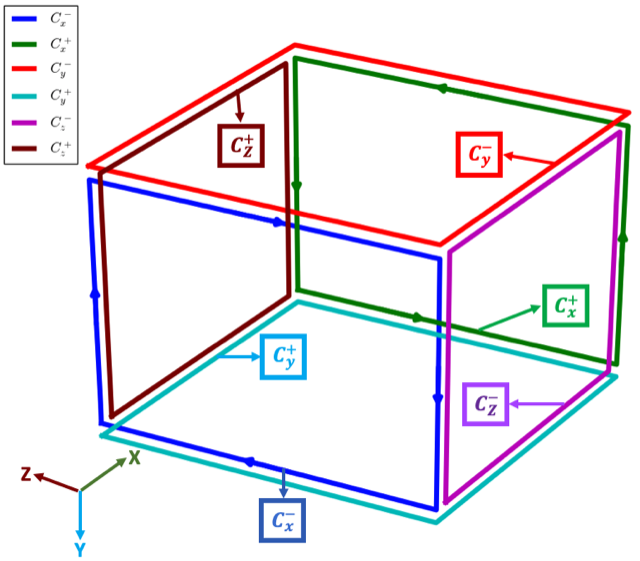
\includegraphics[scale=.28]{Images/c1}
        \caption{Current Direction in $C_x^{\pm}$}
        \label{fig:c1}
    \end{subfigure}%
    \begin{subfigure}{.5\linewidth}
        \centering
        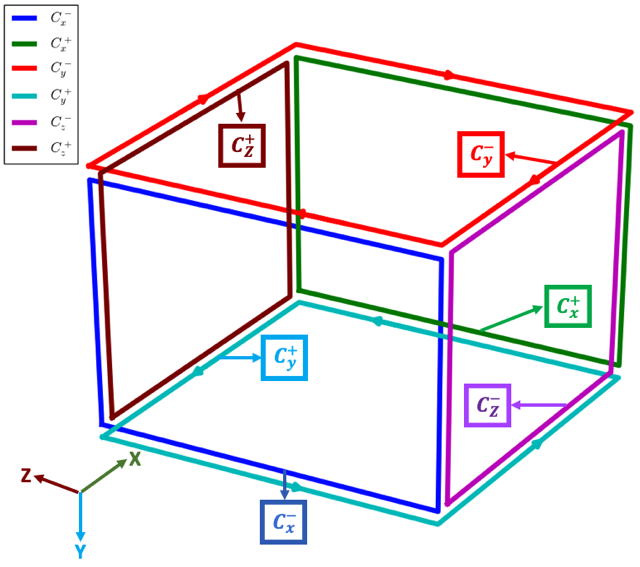
\includegraphics[scale=.28]{Images/c3}
        \caption{Current Direction in $C_y^{\pm}$}
        \label{fig:c3}
    \end{subfigure}\\[1ex]
    \begin{subfigure}{\linewidth}
        \centering
        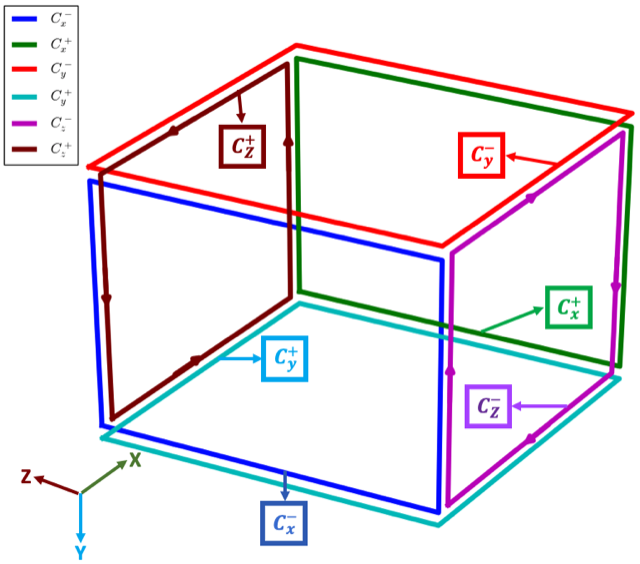
\includegraphics[scale=.33]{Images/c5}
        \caption{Current Direction in $C_z^{\pm}$}
        \label{fig:c5}
    \end{subfigure}
    \caption[short]{Current direction in $C_x^{\pm}$, $C_y^{\pm}$ and $C_z^{\pm}$ . The net current is zero while adding the current contribution from all the six coils for this orientation. $C_z^{\pm}$ coils have been wired together to break the configuration which results in significant decrease in matrix condition number. }
    \label{fig:cDir}
\end{figure}

% As previously discussed in Section~\ref{sec:prototype}, there are six compensation coils ($\bm{C_x^\pm}$, $\bm{C_y^\pm}$ and $\bm{C_z^\pm}$) and one perturbation coil ($\bm{P_z^+}$). 
 It can be as explained by Fig.~\ref{fig:cDir} where one of the coil current mode was shown for all six coils. The total current contribution is found to be zero due to current contributions from $C_x^{\pm}$ in Fig.~\ref{fig:c1}, $C_y^{\pm}$ in Fig.~\ref{fig:c3} and $C_z^{\pm}$ in Fig.~\ref{fig:c5}. To break the mode, two out of the six coils have been wired together so that they can act as one resulting total compensation coils be five. 
%It was found that due to this, the condition number is decreased drastically to 2.


